\documentclass[12pt,a4paper,twoside,open=right,bibliography=totoc]{scrbook}
\usepackage{a4wide}
\linespread{1.359140914229522617680} 
\usepackage[utf8]{inputenc}
\usepackage[T1]{fontenc}
\usepackage[english,main=ngerman]{babel}
%\usepackage{bibgerm}
%\usepackage{breakcites} %use?
%\usepackage{cite}
\usepackage[square]{natbib} %[nonamebreak] verwenden?
\renewcommand{\cite}{ \citep}
\usepackage{ziffer}		% deutsches Ziffernformat
\usepackage{units}		% Zahlen mit Einheiten
\usepackage{amsmath}	% Mathematische Formels
\usepackage{amssymb}	% Mathematische Symbole
\usepackage{commath}	% Diffenrenziale
\usepackage{titling}	% Stellt \thedate, \theauthor, \thetitle zur verfügung
\usepackage{placeins}	% stellt FloatBarrier zur verfügung. [section] verwenden?
\usepackage{microtype}	% typographische Verbesserungen
\setkomafont{disposition}{\normalcolor\bfseries}
\usepackage{graphicx}	% Grafiken
\usepackage[format=hang,font={it,footnotesize},labelfont=bf]{caption} % Bildunterschriften
\usepackage{hyperref}	% Weblinks
\hypersetup{
    bookmarks=true,
    pdftoolbar=true,
    pdfmenubar=true,
    pdffitwindow=false,
    pdfstartview={FitH},
    pdftitle={Das Nizza-Modell},
    pdfauthor={Michael F. Sch\"onitzer},
    pdfsubject={Das Nizza-Modell},
    pdfkeywords={Nizza-Modell},
    pdfnewwindow=true,
    colorlinks=true,
    linkcolor=black,
    citecolor=black,
    filecolor=black,
    urlcolor=blue
}

\author{Michael F. Schönitzer}
\title{Das Nizza-Modell}
\newcommand{\theenglishtitle}{The Nice Model}
\date{\today}


\newcommand{\refsec}[1]{siehe Kapitel~\ref{#1}}
\newcommand{\degree}{$^\circ$}
%\newcommand{\AU}{\,\mathrm{AU}}
\newcommand{\ME}{M_\oplus}
\renewcommand{\vec}{\mathbf}
\renewcommand{\H}{\mathcal H}
\newcommand{\aj}{The Astronomical Journal}
\newcommand{\apj}{The Astrophysical Journal}
\newcommand{\icarus}{Icarus}
\newcommand{\apjl}{The Astrophysical Journal Letters}

%%%%%%%%%%%%%%%%%%%%%%%%%%%%%%%%%%
\newcommand\abstractname{Abstract}  %%% here
\makeatletter
\if@titlepage
  \newenvironment{abstract}{%
      \titlepage
      \null\vfil
      \@beginparpenalty\@lowpenalty
      \begin{center}%
        \bfseries \textsc{\abstractname}
        \@endparpenalty\@M
      \end{center}}%
     {\par\vfil\null\endtitlepage}
\else
  \newenvironment{abstract}{%
      \if@twocolumn
        \section*{\abstractname}%
      \else
        \small
        \begin{center}%
          {\bfseries \textsc{\abstractname}\vspace{-.5em}\vspace{\z@}}%
        \end{center}%
        \quotation
      \fi}
      {\if@twocolumn\else\endquotation\fi}
\fi
\makeatother
%%%%%%%%%%%%%%%%%%%%%%%%%%%%%%%%%%

\begin{document}
%\frontmatter
\begin{titlepage}
%\setcounter{page}{0}
\thispagestyle{empty}
\vglue  2 true cm
\centerline{\huge \thetitle}
\vglue  1 true cm
\centerline{\huge \theenglishtitle}
\bigskip\bigskip 
\vglue  2 true cm

\begin{centering}\large
Bachelorarbeit\\
an der Fakultät für Physik\\
der Ludwig-Maximilians-Universität München
\\[1cm]
vorgelegt von\\
\theauthor\\
geboren in München am 5.4.1990\\
\end{centering}
\vglue  6 true cm
\centerline{\theauthor}
\centerline{\today}
\end{titlepage}

%\addchap*{Abstract}
\begin{abstract}
Das Nizza-Modell betrachtet das Sonnensystem, nachdem sich die Gasscheibe bereits aufgelöst hat, das Sonnensystem besteht nun aus der Sonne, den Planeten und einer Scheibe von Planetesimalen. Das Modell geht in Übereinstimmung mit Planetenentstehungsmodellen davon aus, dass die Planeten damals nahezu kreisförmige, kompakte Orbits hatten.

Aus dieser Scheibe werden von den Riesenplaneten immer wieder einzelne Planetesimale gestreut.
Dabei kommt es durch die Impulsübertragung zu einer Änderung der Planeten\-orbits\cite{Tsiganis2005},
wodurch Saturn, Uranus und Neptun langsam nach außen wandern, während Jupiter langsam nach innen wandert\cite{Hahn1999,Tsiganis2005}.
Mit der Zeit kommen sich die Planeten durch die Migration näher und es kommt zu einer Resonanz,
welche zu einer schlagartigen Erhöhung der Exzentrizitäten der Umlaufbahnen von Jupiter und Saturn, auf Werte die mit den heutigen vergleichbar sind, führt.
Die Planeten Saturn, Uranus und Neptun kommen sich gegenseitig und der Scheibe aus Planetesimalen nahe. Dadurch werden die Planetesimale praktisch schlagartig zerstreut, das System wird instabil und ein Teil der Planetesimale fliegt in das innere Planetensystem und löst dort das Late Heavy Bombardment aus.
Einige der Planetesimale werden auf Orbits um die Lagrangepunkte der Planeten oder um die Planeten selbst gefangen und bilden somit die Trojaner beziehungsweise irregulären Satelliten.

Nach etwa hundert Millionen Jahren erreichen die Planeten schließlich ihre heutigen Entfernungen, ihre Exzentizitäten werden gedämpft und das System stabilisiert sich wieder. Die übriggebliebenen Planetesimale bilden die heutigen transneptunischen Objekte.
\end{abstract}

\cleardoublepage
\setcounter{page}{1}
\tableofcontents
\clearpage
%\mainmatter

\chapter{Einleitung}
Das heutige Standardmodell der Stern- und Planetenentstehung geht von einem Gravitationskollaps in einer großen molekularen Wolke aus, die auf 99\% Wasserstoff- und Heliumgas sowie etwa $\unit[0,1]{\mu m}$ großen Staubteilchen besteht\cite{Hanslmeier2002}. Es entsteht ein Protostern in mitten der sich durch die Drehimpulserhaltung zunächst immer schneller drehenden und dadurch abgeplatteten Gasscheibe.
Später wird der Drehimpuls nach außen transportiert. % durch was
Durch die Brown'sche Bewegung kommt es zu zufälligen Zusammenstößen in der Gaswolke, wodurch die Teilchengrößen anwächst. Diese wachsen durch Akkretion von Gas und später durch Kollisionen weiter bis hin zu etliche Kilometer großen Klumpen, Planetesimale genannt.
Diese wachsen durch den gravitativen Einfang von kleineren Planetesimalen immer stärker bis sie ihre Umgebung gravitativ dominieren und man dann von planetaren Embryonen spricht.

Während man früher annahm, dass die Planeten ungefähr auf ihren heutigen Bahnen entstanden, ist seit \cite{Goldreich1979,Goldreich1980} bekannt, dass es 
durch die Wechselwirkung der planetaren Embryos mit der Gasscheibe in die sie noch immer eingebettet sind, es zu einer Veränderung des Planeten-Orbits, genant Migration, kommt.
Diese Migration entsteht durch zwei Effekte:
\begin{itemize}
\item Lindblad-Drehmoment: Die Gasscheibe umkreist den Stern, im Gegensatz zum Planeten, nicht mit der Keplergeschwindigkeit; durch die unterschiedlichen Geschwindigkeiten kommt es zu Dichtewellen in der Gasscheibe und es entstehen asymmetrische, vom Planeten weglaufende Spiralarme. Durch diese Asymmetrie kommt es zur Drehimpulsübertragung vom Planeten zur Scheibe und somit zur Verringerung der großen Halbachse.
\item Corotation-Drehmoment: Durch die Wechselwirkung mit Gas, welches auf dem selben Orbit kreist, kommt es meist zu einer Drehimpulszunahme.
\end{itemize}
Analytische Berechnungen und Hydrodynamische Simulationen zeigten, dass diese Migration der Riesenplaneten im allgemeinen nach innen gerichtet ist.
Gleichzeitig stabilisiert die Gasscheibe die Planetenbahnen, auch wenn sie sich in Bahnresonanzen befinden, und dämpfen die Exzentrizitäten.
Zum Zeitpunkt als sich nach einigen Millionen Jahren die Gasscheibe auflöst befinden sich die Planeten auf engen, kompakten, kreisförmigen Orbits, welche sich meist in sogenannten Mean-Motion-Resonanzen (\refsec{resonanzen}) zueinander befinden\cite{Nesvorny2011}.
Dies erklärt die Beobachtung von zahlreichen Hot Jupiters und Mean-Motion-Resonanzen in Exoplanetensystemen.

Da sich die Planeten\footnote{Sofern nicht anderes angegeben, betrachten wir im folgenden immer nur die vier Gasriesen Jupiter, Saturn, Uranus und Neptun. Die terrestrischen Planten sind aufgrund der geringen Masse vernachlässigbar.} im heutigem Sonnensystem und bei anderen Planetensystemen auf weiter entfernten Bahnen befinden, braucht es einen Mechanismus, welcher die Planeten wieder auf weiter entfernte Bahnen bringt.
Dies geschieht durch die Bahnresonanzen welche nun nicht mehr durch die Gasscheibe stabilisiert werden.
Durch sie wird das System instabil und die Planeten streuen sich gegenseitig.

Im Jahr 2005 veröffentlichen Gomes, Levison, Morbidelli und Tsiganis drei Nature-Artikel\cite{Tsiganis2005,Morbidelli2005,Gomes2005},
in denen sie ein neues Modell vorstellten, dass genau dies für unseres Sonnensystem beschreibt.
Dieses Modell ist außerordentlich erfolgreich und wird Nizza-Modell genannt, da die Autoren zu besagter Zeit am \emph{Observatoire de la Côte d’Azur} in Nizza arbeiteten.

\FloatBarrier
\chapter{Grundlagen}
Zunächst wollen wir ein paar für das Verständnis des Nizza-Modells notwendige Grundlagen betrachten.

Beim Nizza-Modell betrachten wir die Entwicklung der Planetenbahnen unter Be\-rück\-sich\-ti\-gung der gegenseitigen gravitativen Einflüsse der Planeten -- es handelt sich hier somit um klassische Himmelsmechanik.
Wir betrachten dabei ein $n$-Körperproblem mit $n>2$ Teilchen, welche lediglich gravitativ wechselwirken.
Der Hamiltonian des $n$-Körperproblems lautet bekannterweise
\begin{equation}\label{eq:nbodyhamilton}
{\mathcal H} = \sum\limits_{i=0}^{n-1} \frac{\vec p_i^2}{2m_i} - \sum\limits_{i<j} \frac{Gm_im_j}{r_{ij}}
\end{equation}
wobei $r_{ij}=\norm{\vec q_i-\vec q_j}$ der Abstand der Teilchen $i$ und $j$ ist. % Mehr Symbole erklären?
Bei gegebenen Anfangswerten bestimmt der Hamiltonian durch die hamiltonschen Bewegungsgleichungen
\begin{equation}
\vec{\dot{q}}_i = \pd{\mathcal H}{\vec p_i} \quad ; \quad \vec{\dot{p}}_i = - \pd{\mathcal H}{\vec q_i}
\end{equation}
die zukünftige Entwicklung des Systems. Zur Notation sei vermerkt, dass im folgenden $\vec q$ und $\vec p$ die $3n$ Orte und Impulse aller Teilchen darstellen.

\section{Numerische Integratoren}
Während die das Zweikörperproblems durch die Keplerschen Gesetze analytisch gelöst ist, ist das $n$-Körperproblem bereits ab drei Teilchen nicht mehr allgemein analytisch lösbar.
Zwar sind analytische Näherungslösungen unter gewissen Voraussetzungen möglich, jedoch verlieren diese ihre Gültigkeit, wenn man versucht die Dynamik des Systems über sehr lange Zeiträume zu betrachten. Stattdessen verwendet man dafür numerische Computersimulationen.
Doch auch hier wird die Zeitspanne, die Genauigkeit und die Anzahl der Teilchen durch die begrenzte Rechnerleistung limitiert.
In den letzten Jahrzehnten sind die Möglichkeiten derartiger Computersimulationen jedoch rasant gewachsen. So ist die Zeitdauer über welche das Sonnensystem integrierbar ist, seit den 1960er Jahren von einigen $10^4$ auf über $10^9$ Jahre – das entspricht dem Alter des Sonnensystems – gestiegen. Ein Grund dafür ist natürlich die rasant steigende Rechenleistung der Computersysteme, ein ähnlich großer Effekt kam jedoch durch die Verbesserung der Simulationsalgorithmen\cite{Morbidelli2002}. Im Folgenden möchte ich die Funktionsweise derartiger Algorithmen grundlegend erklären und die Konzepte erläutern, welche hinter diesen bahnbrechenden Verbesserungen stehen. Dabei werde ich mich auf die für die Himmelsmechanik wesentlichen Punkte aus physikalischer Sicht beziehen -- eine detailliertere, allgemeinere Betrachtung aus Sicht der Mathematik und Informatik soll hier nicht beschrieben werden.
Für eine ausführlicherer Betrachtung der historischen Entwicklung und Bedeutung der Integratoren sei auf die lesenswerte Arbeit von \cite{Morbidelli2002} verwiesen.

Herzstück eines jeden Algorithmus zur numerischen Integration ist ein sogenanntes Mapping. Ein Mapping ist ein mathematisches Objekt der Art
\begin{equation}
a_{n+1} = F(n,a_0,...,a_n) \,,
\end{equation}
also eine Vorschrift wie man aus vergangenen Werten einer Folge den nächsten Folgenwert berechnet. Für eine allgemeine Betrachtung von Mappings auf Himmelsmechanischer Sicht sei auf \cite{Dvorak2005} verwiesen.
Was wir nun suchen ist ein Mapping, dass bei gegebenen Punkt im Phasenraum $\vec{w}\equiv(\vec{q},\vec{p})$ zum Zeitpunkt t den Punkt im Phasenraum $\tilde{w}$ bestimmt, welcher den wahren Zustand des Systems zum Zeitpunkt $t'=t+h$ möglichst genau approximiert und dabei trotzdem möglichst einfach berechnet werden kann\cite{Binney2008}.

Ein Trick, der dafür hilfreich ist, ist das \textit{averaging principle}: dieses besagt, dass periodische Oszillationen, deren Dauer klein im Vergleich zur Schrittweite $h$ des Algorithmus ist, sich heraus mitteln und daher das Langzeitverhalten nur unwesentlich verfälschen\cite{Wisdom1991}.
Beschränken wir uns zunächst der Einfachheit halber auf Hamiltonians der Form $\mathcal H(\vec q,\vec p)= \frac{1}{2}\vec p^2+\Phi(\vec q)$.
Durch das averaging principle können wir den Hamiltonian nun um periodisch oszillierende Terme
\begin{equation}
\delta_h(t) = \sum\limits_{n=-\infty}^{\infty} \cos(nt\cdot \frac{2\pi}{h}) = h \cdot \sum\limits_{n=-\infty}^{\infty} \delta(t-h n)
\end{equation} % nochmal überprüfen ob die Verallgemeinerung stimmt
ergänzen und erhalten damit den neuen Hamiltonian
\begin{equation}
\mathcal H_h(\vec q,\vec p)= \frac{1}{2}\vec p^2+\Phi(\vec q)\delta_h(t)
\end{equation}
der die selben Orbits liefern sollte, solange $h$ klein genug ist. $\delta_h(t)$ ist dabei eine periodische Serie von Dirac-Funktionen. Die Hamiltongleichungen lauten damit
\begin{equation}
\vec{\dot q} = \pd{\H_h}{\vec{p}} = \vec{p} \quad ; \quad 
\vec{\dot p} = \pd{\H_h}{\vec{q}} = - \vec{\nabla}\Phi(\vec q)\delta_h(t) \, .
\end{equation}
Dies lässt dich jetzt von $t=\epsilon$ bis $t=h+\epsilon$ mit $0 < \epsilon \ll h$ integrieren. Dazu integrieren wir zunächst von $t=\epsilon$ bis $t=h-\epsilon$, in diesem Zeitraum ist die Deltafunktion Null, somit bleibt der Impuls konstant. Der Ort verändert sich somit linear, was dem Schritt den Namen \textit{drift step} verleiht:
\begin{equation}
\bar{\vec{q}} = \vec{q}+h\vec{p} \quad ; \quad \bar{\vec{p}} = \vec{p}
\end{equation}
Danach folgt das Zeitintervall von $t=h-\epsilon$ bis $t=h+\epsilon$. Hier ändert sich der Ort für $\epsilon\to 0$ nur infinitesimal, der Impuls erhält jedoch einen Stoß
\begin{equation}
\vec{q'}=\vec{\bar{q}} \quad ; \quad \vec{p'}=\vec{\bar{p}}-h\vec{\nabla}\Phi(\vec{q'})
\end{equation}
dies nennt man den \textit{kick step}. Zusammen bilden diese Schritte den \textit{modifizierten drift-kick Euler Integrator}\cite{Binney2008}.
Das Mapping für diesen lautet also
\begin{equation}
\vec{q'}=\vec{q}+h\vec{p} \quad ; \quad \vec{p'}=\vec{p}-h\vec{\nabla}\Phi(\vec{q'})\,.
\end{equation}
Für das Verständnis halte ich es für sehr wichtig, noch eine zweite, zum Ansatz über das averaging principle alternative, Betrachtungsweise für dieses Mapping zu erläutern.
Für eine beliebige Observable $f(\vec q(t),\vec p(t))$ gilt bekanntermaßen:
\begin{align}
\od{f}{t} &= 
\sum_{k=0}^{3n-1} \left(
	\pd{f}{q_k} \pd{q_k}{t} +
	\pd{f}{p_k} \pd{p_k}{t}
\right) \\ &=
\sum_{k=0}^{3n-1} \left(
	\pd{f}{q_k} \pd{\H}{p_i} +
	\pd{f}{p_k} \pd{\H}{q_i}
\right) \\ &=
\lbrace f,\H \rbrace \\ &=:
O_\H f \label{eq:Of}
\end{align}
wobei $O_\H$ ein Operator ist. Die allgemeine Lösung für Gleichung \ref{eq:Of} kann mit der Exponentialfunktion geschrieben werden als:
\begin{equation}
f(t+h) = e^{hO_\H}f(t)
\end{equation}
Wird nun der Hamiltonian in zwei Teile gespalten $\H=\H_A+\H_B$, so ergibt sich $f$ aus
\begin{equation}
f(t+h)=e^{h\left(O_A+O_B\right)}f(t)
\end{equation}
wobei $O_A=\lbrace f, H_A \rbrace$ und $O_B=\lbrace f, H_B \rbrace$ nicht kommutierende Operatoren sind\cite{Chambers1999}. Betrachten wir die die Exponentialfunktion bis zum quadratischen Term
\begin{equation}
e^{h\left(O_A+O_B\right)} = 1 + h\left(O_A+O_B\right) + \frac{h^2\left(O_A^2+O_AO_B+O_BO_A+O_B^2\right)}{2} + ... \label{eq:OAB}
\end{equation} % das O ist scheißhäßlich, doch Notation von Chambers übernehmen
vergleicht man das nun mit dem hintereinander ausführen der beiden Operatoren
\begin{equation}
e^{hO_A}e^{hO_B} = 1 + h\left(O_A+O_B\right) + \frac{h^2\left(O_A^2+2O_AO_B+O_B^2\right)}{2} + ... \label{eq:OA+B}
\end{equation}
Die beiden stimmen also in erster Ordnung miteinander überein, erst in zweiter Ordnung gibt es Abweichungen aufgrund der nicht kommutierenden Operatoren\cite{Chambers1999}. Das Anwenden eines der Exponentialoperatoren auf die Größe $f$ entspricht dem Bestimmen der Bewegungsgleichungen unter Beachtung von nur der entsprechenden Hälfte des Hamiltonians.
Ein symplektischer Integrator erster Ordnung löst die Bewegungsgleichungen also dadurch annähernd, das er zuerst $\H_B$ und anschließend $\H_A$ anwendet.
Der Fehler des Integrators ist also von der Ordnung $\mathcal{O}(h^2)$.
Genau dies geschieht auch bei dem oben beschriebenen modifizierten drift-kick Euler Integrator,
wo wir zunächst über den Zeitrum $h$ die Auswirkung der kinetischen Energie $\H_p=\frac{1}{2}\vec{p}$ und anschließend über den selben Zeitraum $h$ die Auswirkung der potentiellen Energie $\H=\Phi(\vec{q})$ anwendeten.

Eine deutliche Verbesserung der Genauigkeit lässt sich erreichen, indem man noch die zweite Ordnung von Gleichung \ref{eq:OAB} und \ref{eq:OA+B} berücksichtigt. Ein solcher Integrator zweiter Ordnung wendet zunächst für eine Dauer von $h/2$ den ersten Teil des Hamiltonians an, dann für die Zeitdauer $h$ den zweiten und schließlich wieder für die Zeit von $h/2$ den ersten Teil an:
\begin{equation}
q(t+h)=e^{hO_B/2}e^{hO_A}e^{hO_A/2} \label{eq:secondorder}
\end{equation}
Wendet man dies auf die obige Aufteilung des Hamiltonians in kinetische und potentielle Energie an, so erhält man den bekannten Leapfrog-Integrator\cite{Duncan1998}. Der Fehler dieser Integratoren ist $\mathcal{O}(h^3)$ fällt also für kleine Schrittweiten deutlich schneller ab\cite{Chambers1999}.
Es ist nun möglich noch höhere Ordnungen mit einzubeziehen, damit wird der Integrator bei gleicher Schrittweite immer genauer, beziehungsweise die nötige Schrittweite für eine gewünschte Genauigkeit wird immer größer. Gleichzeitig werden jedoch die Mappings immer komplizierter, weshalb jeder einzelne Schritt immer rechenzeitaufwendiger zu berechnen wird. Integratoren höherer Ordnung sind deshalb meist nicht schneller als Integratoren der zweiten Ordnung\cite{Chambers1999}.

Für die Simulation des Sonnensystems über lange Zeiträume sind symplektische Integratoren von besonderer Bedeutung. Symplektische Integratoren sind Algorithmen die die Zweiform $\dif p \wedge \dif q$ erhalten, vereinfacht gesagt bedeutet das, dass der Integrator das Phasenraumvolumen erhält\cite{Duncan1998}. Dies führt dazu, dass es bei symplektischen Integratoren keinen Drift der Energie gibt, sondern die Energie auch über beliebig lange Zeiträume konstant ist\cite{Binney2008}. Darüber hinaus sind sie meist zeitreversibel, wendet man also einen Zeitschritt $t\to t+h$ und anschließend einen Zeitschritt $t+h\to t$ an, so erhält man bis auf Rundungsfehler den exakt selben Punkt im Phasenraum\cite{Duncan1998}.
Da wir das Mapping von obigen modifizierten Euler Integrator direkt aus dem Hamiltonian hergeleitet haben, handelt es sich hier um einen einfachen symplektischen Integrator\cite{Binney2008}.

1991 beschrieben \cite{Wisdom1991} einen symplektischen Integrator, welcher zu einer revolutionären Verbesserung der Möglichkeiten zur Simulation des Sonnensystems führte.
Man nennt diesen und verwandte Algorithmen \textit{mixed variables Symplectic} (MVS) Integratoren. 
Weite Verbreitung fand der Algorithmus von Wisdom und Holman vor allem durch die Implementation namens Swift durch \cite{Levison1994}.
Auf dem Prinzip dieses Integrators basieren auch die auch die für das Nizza-Modell relevanten Codes, weshalb ich diesen hier erläutern werde.

Die grundlegende Eigenschaft des Sonnensystems, die hier genutzt wird, ist, dass die Masse der Sonne die der Planeten deutlich überwiegt und die Planeten sich deshalb annähernd auf Keplerschen Planetenbahen bewegen. Man spaltet nun den Hamiltonian in zwei Teile auf:
\begin{equation}
\H = \H_{\mathrm{Kepler}} + \H_{\mathrm{Interaktion}}
\end{equation}
Wobei $\H_{\mathrm{Kepler}}$ die Bewegung der Planeten um den Zentralkörper und $\H_{\mathrm{Interaktion}}$ die Beeinflussung der Körper untereinander beschreibt. Während solch eine Zerlegung in analytischen Theorien im Rahmen von Störungsrechnungen nichts ungewöhnliches ist, war dieser Ansatz vor Wisdom und Holman in nummerischen Verfahren nicht gebräuchlich\cite{Wisdom1991}. Hat man den Hamiltonian so aufgeteilt, kann man wie schon oben durch das Hinzufügen von periodischen Funktionen einen Mapping-Hamiltonian finden:
\begin{equation}
\H_{\mathrm{Map}} = \H_{\mathrm{Kepler}} + \H_{\mathrm{Interaktion}}\delta_{2\pi}(\Omega t)
\end{equation} % Was ist Omega?
Das Integrieren zu den Zeiten zwischen den Peaks ist einfach möglich, die Lösungen sind natürlich die Keplerschen Bahnen. Das Integrieren über die Peaks ist ebenfalls möglich, da hier analog zu oben $\H_{\mathrm{Kepler}}$ nichts beiträgt und die Deltafunktion das Auswerten des Integrals bekanntermaßen erheblich vereinfacht\cite{Wisdom1991}. %are you kidding?
Nun gilt es also den Hamiltonian des $n$-Körperproblems \ref{eq:nbodyhamilton} in $\H_{\mathrm{Kepler}}$ -- bestehend aus voneinander unabhängigen Keplerschen Hamiltonians -- sowie einen Interaktions Hamiltonian auf zu teilen. Ein Keplerscher Hamiltonian ist dabei ein Hamiltonian der Form
\begin{equation}
\H = \frac{p^2}{2m} - \frac{\mu}{r} \,.
\end{equation}
\begin{figure}[tbn]
\centering
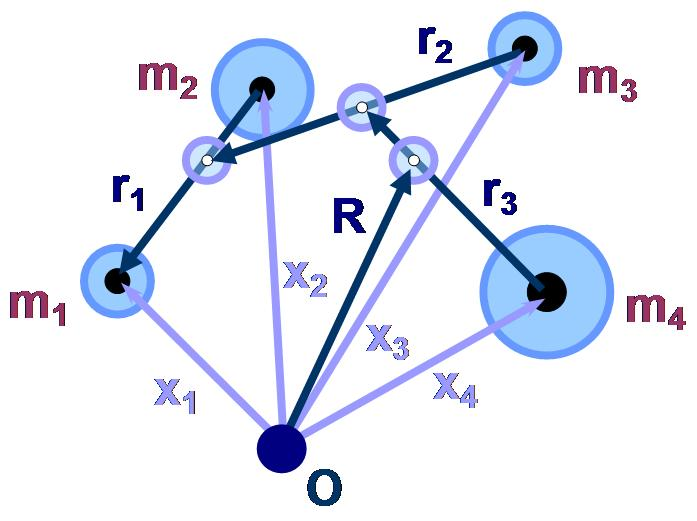
\includegraphics[scale=0.5]{img/Four-body_Jacobi_coordinates} % in SVG umwandeln
\caption{Jacobi Koordinaten veranschaulicht für 4 Körper. Hellblau sind jeweils die virtuellen Massen eingezeichnet. Die Jacobi Koordinaten sind $r_1$, $r_2$, $r_3$ und $R$. Bild: Brews ohare, CC-BY-SA.}
\label{fig:Jacobi}
\end{figure}
Für ein Zweiteilchensystem ist offensichtlich, dass man die gewünschte Form erreicht, indem man das System in den Koordinaten relativ zum Schwerpunkt schreibt. Für $n$ Teilchen erhält man den Effekt durch Verwendung der Jacobi-Koordinaten, diese erhält man wie folgt.
Wir betrachten die Massenpunkte $m_j$ und $m_k$, diese ersetzen wir durch einen virtuellen Massenpunkt $m_{jk}$ am Ort des Schwerpunktes der Massen $R_{jk} = (m_j q_j + m_k q_k)/(m_j + m_k)$ und erhalten den Relativabstand $r_{jk} = x_j - x_k $.
Wir iterieren diese Verfahren nun mit den restlichen $n-2$ Massenpunkten, sowie dem neuen virtuellen Massenpunkt. Am Ende haben wir $n-1$ relative Koordinaten $r_{ik}$ sowie den zuletzt berechneten $R_{1n}$ welcher die Koordinate des Schwerpunkts des Systems angibt.
Abbildung \ref{fig:Jacobi} verdeutlicht das Vorgehen.
In Formeln ausgedrückt lauten die, im folgenden gestrichen geschriebenen, Jacobi-Koordinaten:
\begin{align}
x'_0 &= \frac{1}{M} \sum\limits_{j=0}^{n-1} m_j\vec{x}_j \\
x'_{i\neq0} &= x_i - X_{i-1}
\end{align}
mit
\begin{equation}
X_i = \frac{1}{\eta_i} \sum\limits_{j=0}^{i} m_j\vec{x}_j
\end{equation}
und
\begin{equation}
\eta_i = \sum\limits_{j=0}^{i} m_j \quad ; \quad M = \eta_{n-1}\,.
\end{equation}
Die dazugehörigen transformierten Massen und Impulse sind:
\begin{equation}
m_0 = M \quad ; \quad m'_{i\neq 0} = m_i \frac{\eta_{i-1}}{\eta_{i}} \quad ; \quad p'_i = m'_i v'_i
\end{equation}
Setzt man dies in \ref{eq:nbodyhamilton} ein, so erhält man nach einigen Umformungen: %durchrechnen, vorrechnen?
\begin{equation}
\H = \frac{p'^2_0}{2M} + \sum\limits_{i=1}^{n-1} \frac{p'^2_i}{2m'_i} - \sum\limits_{i=1}^{n-1} \frac{Gm_im_0}{r_{i0}} - \sum\limits_{0<i<j} \frac{Gm_im_j}{r_{ij}}
\end{equation}
wobei $r_{ij}=\norm{\vec{x}_i-\vec{x}_j}$ der Abstand zweier Körper ist. Der erste Term beschreibt die Bewegung des Schwerpunktes, welche – wie zu erwarten war – die eines freien Teilchens ist. Da wir uns für die Planetenbahnen, nicht aber für die Eigenbewegung des gesamten Sonnensystems interessieren, können wir diesen Term ignorieren.
Wir formen den Hamiltonian weiter um, indem wir den Term
\begin{equation}
\sum\limits_{i=1}^{n-1} \frac{Gm_im_0}{r'_i}
\end{equation}
einmal mit positiven und einmal mit negativen Vorzeichen einfügen:
\begin{equation}
\H = \sum\limits_{i=1}^{n-1} \left( \frac{p'^2_i}{2m'_i} - \frac{Gm_im_0}{r'_i} \right)
  +  \sum\limits_{i=1}^{n-1} \left( \frac{Gm_im_0}{r'_i} - \frac{Gm_im_0}{r_{i0}} \right)
  -  \sum\limits_{0<i<j} \frac{Gm_im_j}{r_{ij}}
\end{equation}
Wie man sieht ist der erste Term nun wie gewünscht eine Summe von $n-1$ voneinander unabhängigen Keplerschen Hamiltonians. Die beiden anderen Summen bilden $\H_{\mathrm{Interaktion}}$ und ist deutlich kleiner als $\H_{\mathrm{Kepler}}$. Unser Mapping Hamiltonian lautet also zusammenfassend:
\begin{align}
\H_{\mathrm{Map}} &= \H_{\mathrm{Kepler}} + \H_{\mathrm{Interaktion}}\delta_{2\pi}(\Omega t) \\
\H_{\mathrm{Kepler}} &= \sum\limits_{i=1}^{n-1} \left( \frac{p'^2_i}{2m'_i} - \frac{Gm_im_0}{r'_i} \right) \\
\H_{\mathrm{Interaktion}} &= \sum\limits_{i=1}^{n-1} \left( \frac{Gm_im_0}{r'_i} - \frac{Gm_im_0}{r_{i0}} \right)
  -  \sum\limits_{0<i<j} \frac{Gm_im_j}{r_{ij}}
\end{align}
Wie bereits besprochen ist dieser Mapping Hamiltonian über den Zeitschritt $t \to t+h$ analytisch lösbar und liefert somit ein Mappig das zur Simulation des Systems verwendet werden kann.
Das soeben beschriebene Verfahren entspricht wieder einem Integrator erster Ordnung, der Fehler ist also von der Ordnung $\mathcal{O}(h^2)$.
Erinnern wir uns nun an die Gleichungen \ref{eq:OA+B} und \ref{eq:OAB} zurück, so finden wir, dass sich der Fehler zu
\begin{equation}
e^{hO_A}e^{hO_B}-e^{h\left(O_A+O_B\right)} = \frac{h^2}{2} \left( O_AO_B-O_BO_A \right) + ...
\end{equation}
ergibt. Dabei sind auch alle höheren Terme von A und B abhängig\cite{Chambers1999}. Für ein System für das gilt $O_B\sim\epsilon O_A$ mit kleinem Epsilon, so ist der Fehler auch proportional zu $\epsilon$.
Da die Sonne fast 99,9 Prozent der Masse des Sonnensystems besitzt, %Quelle?
gehorchen die Planetenbahnen in sehr guter Annäherungen den Keplerschen Gesetzen und $\H_{\mathrm{Kepler}}$ dominiert deutlich über $\H_{\mathrm{Interaktion}}$. Die Genauigkeit des Integrators ist somit $\mathcal{O}(h^2\epsilon)$, sie ist also bei gleicher Schrittweite um mehrere Größenordnungen höher als bei dem einfacheren modifizierten Eulerschen Integrator – oder anderes herum: bei gleicher Genauigkeit kann die Schrittweite deutlich größer gewählt werden, was die Integration entscheidend beschleunigt.
Es ist nun möglich auch dieses Verfahren gemäß Gleichung \ref{eq:secondorder} zu einem Integrator zweiter Ordnung  mit Genauigkeit $\mathcal{O}(h^3\epsilon)$ machen. Es sei noch darauf hingewiesen, dass \cite{Saha1992} und \cite{Wisdom1996} Möglichkeiten gefunden haben um den Fehler des Integrators proportional zu $\epsilon^2$ zu machen.
Während man bei einem Leapfrog Integrator für eine hinreichen gute Genauigkeit noch Schrittweiten von $10^{-3}\;T_{\mathrm{min}}$ braucht, wobei $T_{\mathrm{min}}$ die Umlaufzeit des kleinsten Orbits bezeichnet, sind es bei MVS Integratoren typischer weiße $1/20\;T_{\mathrm{min}}$\cite{Duncan1998}. Natürlich wird vieles des Geschwindigkeitsgewinnes wieder dadurch aufgefressen, dass die Berechnung der einzelnen Schritte aufwendiger ist, unterm Strich bleibt jedoch ein signifikanter Geschwindigkeitszuwachs von etwa einer Größenordnung\cite{Chambers1999}.
Eine wichtige Sonderfunktion, die ein guter Integrator unterstützen sollte, sie die der Testteilchen, also Teilchen deren Bewegung zwar von den anderen Teilchen beeinflusst wird, die sich jedoch nicht gegenseitig und auch nicht die anderen Teilchen beeinflussen. Dieses Verhalten entspricht dem Fall, dass die Masse des Teilchens  vernachlässigbar klein wird.
Auch das Mapping von \cite{Wisdom1991} unterstützt nach geeigneten algebraischen Umformungen Testteilchen.
Testteilchen sind aus zwei Gründen von Bedeutung: zum einen, wenn man das Gravitationsfeld eines Systems betrachten will ohne es zu beeinflussen, zum anderen ist wird die Berechnung deutlich schneller, wenn man Teilchen mit kleiner Masse als Testteilchen betrachtet -- dies ist wie wir sehen werden beim Nizza-Modell von zentraler Rolle, da man hier eine Vielzahl an Teilchen hat, deren Masse wesentlich kleiner als die der Planeten ist.
Ein weiterer interessanter Punkt ist, dass obwohl die Reihenfolge der Körper bei der obigen Betrachtung irrelevant war, die Verwendung der natürlichen Reihenfolge, mit steigender großen Halbachse, \glqq sauberere\grqq\ Orbits liefert -- anderenfalls enthalten die Orbits schnelle Oszillationen.
Daneben gibt es natürlich noch einige Aspekte des Algorithmus die optimiert werden können, diese spielen jedoch für das Verständnis der Funktionsweise keine Rolle, daher werde ich auf sie hier nicht eingehen.

Die MVS Integratoren wie der von Wisdom und Holman haben jedoch ein grundlegendes Problem. Die Schrittweite des Integrators wird durch die Wahl der Parameter von $\delta_{2\pi}(\Omega t)$ festgelegt, sie ist also über die ganze Simulation konstant und für alle Planeten gleich.
Dies führt zu mehreren Problemen: Zum einen muss man wenn man, wen man Planeten hat, die auf einen sehr kleinen Orbit den Zentralkörper umkreisen, während andere Planeten sehr große Entfernungen zum Zentralkörper haben die selbe kleine Schrittweite für alle Planeten anwenden, obwohl bei den äußeren wesentlich größere Schrittweiten möglich und sinnvoll wären. Dieses Problem lösten \cite{Saha1994} mit einer Modifikation des Verfahren, welches es erlaubt für jeden Planeten eigene, jedoch weiterhin konstante, Schrittweiten zu wählen.
Dies erhöht die Geschwindigkeit weiter, es löst jedoch zwei andere Probleme noch nicht. Das zweite Problem besteht in einer höheren Ungenauigkeit für Bahnen mit höherer Exzentrizität. Auch dieses Problem konnte durch eine Modifikation des Verfahrens durch \cite{Mikkola1997} überwunden werden.
Das größte Problem jedoch bestand darin, dass sich zwei Planeten nicht zu nahe kommen dürfen, da in diesem Fall $\H_{\mathrm{Interaktion}}$ groß wird und somit das $\epsilon$ nicht mehr klein genug ist. Man würde hier gerne die Schrittweite verkleinern um die Integrationsgenauigkeit zu erhalten, Veränderungen der Schrittweite während der Integration führen jedoch zu Fehlern, da das averaging principle nicht mehr greift.
Bei einzelnen wenigen Planetenbegegnungen ist der Fehler noch klein genug, als das man die Ergebnisse zumindest als statistische Aussagen verwenden kann\cite{Chambers1999},
 spätestens jedoch wenn wir – wie wir es beim Nizza-Modell haben werden – ein sich chaotisch verhaltenes System haben in welchen Plantenbegegnungen sehr häufig vorkommen, ist dieser Ansatz nutzlos.

In den Jahren 1998/1999 erschienen zwei Codes, welche diese Probleme lösten und trotzdem die hohe Geschwindigkeit der MVS Integratoren behielten. Diese sind SyMBA von \cite{Duncan1998} und Mercury von\cite{Chambers1999}. Die beiden Integratoren, welche ähnliche Ansätze haben, sich jedoch in Details unterscheiden, haben das Verständnis von unserem Sonnensystem fundamental weiter gebracht. Sie waren nicht nur Voraussetzung des Nizza-Modells, sondern spielen insbesondere auch für das Verständnis der Planetenakkretion eine wichtige Rolle\cite{Morbidelli2002}.
Anstatt der Jacobi Koordinaten verwenden diese beiden Integratoren kanonische heliozentrische Koordinaten. Bei diesen kreisen die Planeten im Keplerschen Hamiltonian nicht um unterschiedliche Massenzentren, sondern allesamt um die Sonne. Dies hat einerseits zwar den Nachteil, dass die Durchläufe der Planeten durch das Perihel, wenn dieses sehr nahe an der Sonne ist, wie eine Planetenbegegnung betrachtet werden muss, es ist für den Algorithmus jedoch sehr wichtig, dass die Planetenbahnen des Keplerschen Hamiltonians um den selben Punkt rotieren\cite{Morbidelli2002}.
Wann immer sich nun zwei Planeten (oder ein Planet und die Sonne) sich nahe kommen, wird ihre gegenseitige Wechselwirkung nach und nach immer stärker dem Keplerschen Hamiltonian hinzugefügt\cite{Morbidelli2002}.
Dadurch wird der \glqq Keplersche Hamiltonian\grqq\  natürlich analytisch unlösbar und ist auch kein Hamiltonian in Keplerscher Form mehr, seine Auswirkung muss also anderweitig numerisch berechnet werden.
Hier unterscheiden sich die beiden Integratoren nun. Mercury verwendet einen konventionellen Integrator um den \glqq Keplerschen Teil\grqq\  des Hamiltonians zu lösen: den Bulirsch Stoer Integrator mit maximal möglicher Genauigkeit – damit ist gemeint nur beschränkt durch die Rundungsfehler des Rechners\cite{Chambers1999,Morbidelli2002}.
SyMBA hingegen, verwendet auch hierfür wieder einen symplektischen Integrator, mit einer durch eine ganze Zahl geteilten Schrittweite. Wenn die Planeten sich sehr nahe kommen, muss SyMBA das Verfahren iterieren um die Schrittweite noch weiter zu unterteilen\cite{Duncan1998,Morbidelli2002}.

\FloatBarrier

\section{Bahnresonanzen}\label{resonanzen}
Wie in den meisten Gebieten der Physik spielen auch in der Himmelsmechanik Resonanzen eine große Rolle. Sie können ein System entweder stabilisieren oder wie im Fall des Nizza-Modells zu einer rasanten Destabilisierung führen.
Bahnresonanzen treten immer dann auf, wenn zwei Frequenzen eines Systems ein bestimmtes Verhältnis haben.
Die einfachst zu Verstehende und für diese Arbeit wichtigste Bahnresonanz ist die Mean-Motion-Resonanz (MMR), auf deutsch auch Resonanz der mittleren Bewegung, bei welche die Umlaufdauer zweier Körper (in unserem Fall Planeten) im Verhältnis zweier kleiner ganzer Zahlen sind.
Eine 1:2-MMR liegt beispielsweise vor, wenn der eine Planet genau doppelt so lange braucht um den Stern zu umkreisen, als der andere. Betrachtet man nun zwei kreisrunde Planetenorbits in einer gemeinsamen Ebene ($e=i=0$) so kann man leicht verstehen, dass die Planeten sich nach einer Umlaufzeit von $n\cdot 2T$ wobei $T$ die Umlaufdauer des inneren Planeten ist, immer auf der \glqq selben Seite\grqq\ begegnen und die gegenseitige gravitative Wechselwirkung immer in die selbe Richtung wirkt, was dazu führt, dass die Exzentrizität der Planetenorbits steigt. Die 1:2 MMR ist verständlicherweise die stärkste aller Resonanzen.
Die analytische Betrachtung von Mean-Motion-Resonanzen ist möglich, würde aber den Rahmen dieser Arbeit sprengen, der interessierte Leser sei auf \cite{Dvorak2005,Murray2010} verwiesen. % Murray anschauen
Während die MMRs für kreisrunde Orbits nur für exakte Positionen der Planeten eintreten, haben die MMRs eine gewisse endliche Breite sobald die Exzentrizität des Orbits von Null verschieden ist.
%stickyness?
% Beispiele

Ein weiterer wichtiger Typ von Bahnresonanz sind die säkularen Resonanzen – engl. Secular resonances (SR). Sie treten auf wenn die orbitale Präzession zweier Körper synchronisiert sind.
Die Lage eines Orbits im dreidimensionalem Raum, wird neben der Inklination durch die Länge des aufsteigenden Knotens ($\Omega$) und das Argument des Perihels ($\omega$) beschrieben. Die Orientierung dieser Bahnebene schwankt im Laufe der Zeit (Präzession) mit den Fundamentalfrequenzen $g$ und $s$. Säkulare Resonanzen können jetzt als ganzzahliges Vielfaches zwischen einer der Fundamentalfrequenzen, oder einer Linearkombination von $g$ und $s$ sowie der entsprechenden Größe des anderen Planeten auftreten. Auch Linearkombinationen der Fundamentalfrequenzen unterschiedlicher Planeten können zu säkularen Resonanzen führen.
Säkulare Resonanzen führen über ebenfalls lange Zeiträume hinweg zu einer Änderung der Exzentrizität und Inklination der Körper, sind jedoch tendenziell schwächer.

Neben diesen beiden Typen existieren noch eine Reihe weiterer Resonanzen, wie die Kozai-Resonanzen, welche für diese Arbeit jedoch keine größere Rolle spielen. % Kozai erklären?

\section{Dynamische Reibung}
\begin{figure}
\centering
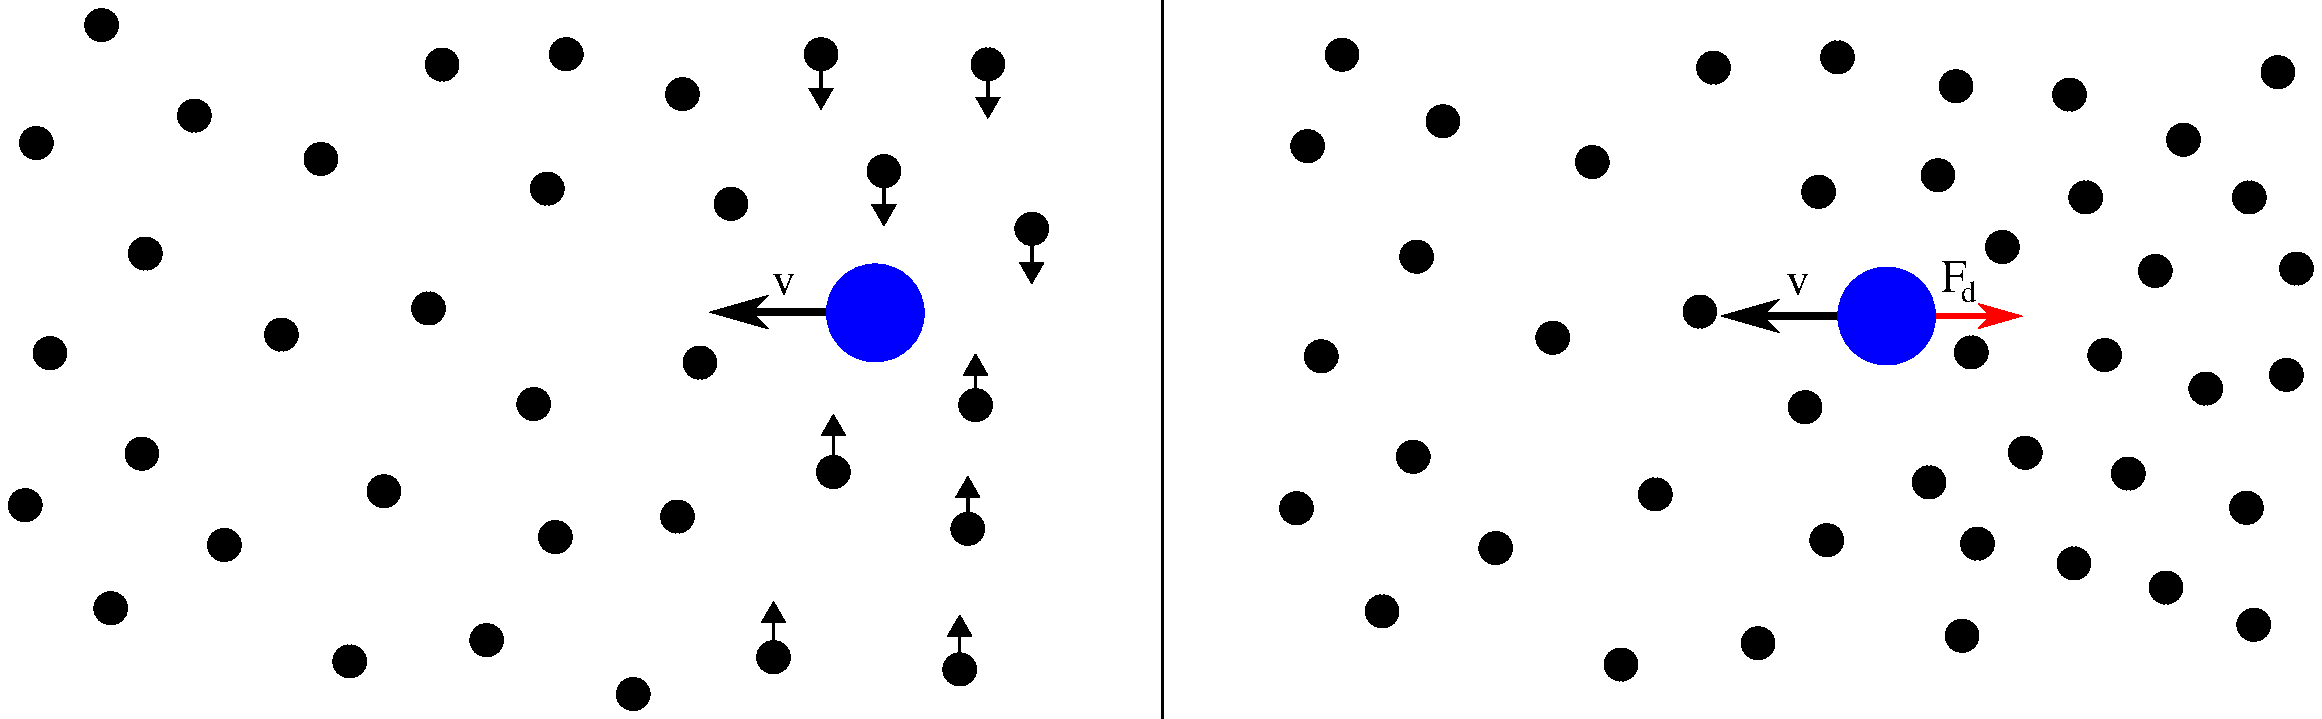
\includegraphics[scale=0.4]{img/dynamischeReibung}
\caption{Fliegt ein Teilchen durch ein Feld von leichteren Teilchen, so werden diese von ihm angezogen. Da sich das Teilchen unterdessen weiterbewegt, kommt es hinter dem Teilchen zu einer erhöhten Dichte, welche das Teilchen durch die gravitative Anziehung abbremst.}
\label{fig:df}
\end{figure}
Ein weiteres Konzept, das wir zum Verständnis des Folgenden benötigen werden, ist das der Dynamischen Reibung (engl. dynamical Friction). Als Dynamische Reibung bezeichnet man die reibungsartige Beeinflussung der Bewegung eines Körpers durch die gravitative Wirkung mit ihn umgebener Materie ohne das es zu eine Berührung mit dieser kommt.
Betrachten wir dazu wie in Grafik \ref{fig:df} dargestellt eine große Masse die sich durch ein Feld vieler zufällig verteilter kleiner Massen bewegt. Der Körper zieht die kleineren Massen nun gravitativ an, so dass diese sich auf ihn zu bewegen und es dort zu einer erhöhten Massedichte kommt. Da sich der Körper inzwischen weiter bewegt hat, kommt es zu einer \glqq Heckwelle\grqq. Durch die gravitative Anziehung dieser \glqq Heckwelle\grqq wird das Teilchen abgebremst.
Näherungsweise kann die Kraft durch Dynamische Reibung auf eine Masse $M$ die sich mit der Geschwindigkeit $v$ durch ein gleichmäßig dichtes Feld (Dichte $\rho$) aus deutlich leichteren Teilchen als
\begin{equation}\label{eq:df}
\textbf{f}_{dyn} \approx C \frac{G^2 M^2 \rho}{v^2_M}
\end{equation}
angegeben werden.

Im folgenden will ich einen Plausibilitätsbeweis dafür liefern, dass die Exzentrizität eines Planetenorbits durch dynamische Reibung reduziert wird.
Bekanntermaßen gilt für die Geschwindigkeit eines sich auf einer Keplerschen Umlaufbahn bewegenden Planeten dessen Masse deutlich kleiner als die der Sonne ist
\begin{equation}\label{eq:Bahngeschwindigkeit}
v= \sqrt{GM\left(\frac{2}{r}-\frac{1}{a}\right)}
\end{equation}
wobei $a$ die große Halbachse ist. Formt man dies nach $r$ um, so erhält man:
\begin{equation}
r = \frac{2aGM}{av^2GM}
\end{equation}
Während einem kleinem Zeitschritt $\Delta t$ beträgt der Betrag der Abbremsung durch die dynamische Reibung gemäß dem Grundgesetz der Mechanik:
\begin{equation}
\Delta v = \frac{f_{dyn}}{M} \Delta t = C \rho \frac{\left(GM\right)^2}{Mv^2} \Delta t
\end{equation}
Diese Abbremsung führt nun zu einer Drift in Richtung Sonne, dessen Größe wir berechnen können:
\begin{equation}
\Delta r = \od{r}{v}\Delta v = \frac{4GMa^2v}{\left(av^2+GM\right)^2} \cdot \Delta v
\end{equation}
durch einsetzen erhalten wir
\begin{equation}
\Delta r = \frac{1}{v} \frac{4a^2G^3M^2 C \rho}{\left(av^2+GM\right)^2}  \Delta t \propto \frac{1}{v^5}
\end{equation} % keine echte Proportionalität
Die Veränderung von $r$ ist also um so stärker, desto langsamer sich das Teilchen bewegt. Nachdem sich nun bekanntermaßen (und auch aus Gleichung \ref{eq:Bahngeschwindigkeit} ablesbar) der Planet um so schneller bewegt, je näher er an diesem ist, können wir daraus schließen, dass er an Sonnenfernen Punkten eine deutlich stärkere Bahnveränderung hin zur Sonne erfährt, als an Sonnennahen. Somit sinkt die Exzentrizität.


\chapter{Das Nizza-Modell}
\section{Die Planetenorbits}\label{Orbits}
Im Folgenden werde ich erklären, wie \cite{Tsiganis2005} mit den Nizza-Modell die Orbits der Planeten erklärte.
Man beginnt die Betrachtung dabei bei dem Zeitpunkt, als die Gasscheibe sich gerade aufgelöst hat.
Als Ausgangszustand wählten die Gruppe um Tsiganis dabei – wie im letzten Abschnitt erläutert – die vier Riesenplaneten auf sehr kompakten Orbits. Zusätzlich nahmen sie an, dass es eine massive Scheibe aus Planetesimalen im Sonnensystem gab -- eine solche ist ein nicht unwahrscheinliches Überbleibsel der Planetenentstehung.

Als Anfangsparameter wählten \cite{Tsiganis2005} in den Simulationen für die große Halbachse des Jupiterorbits $a_J = \unit[5,45]{AU}$ und Saturn wurde wenige Zehntel AU vor der bei $a_{1:2} = \unit[8,65]{AU}$ gelegenen 1:2-MMR gesetzt.
%Dass Saturn weiter innen als auf der zu Jupiter resonanten Bahn war, ist laut \cite{Levison2008} eine notwendige Bedingung, da es anderenfalls schon zu Zeiten der Gasscheibe eine starke Migration durch die Wechselwirkung mit dieser gegeben hätte. %O-Zitat, klarer
Die Orbitalverteilung der transneptunischen Objekte lässt darauf schließen, dass Neptuns Migration innerhalb von 20 AU begonnen hat\cite{Tsiganis2005}.
Deshalb wurden die beiden Eisplaneten zu Beginn der Simulationen auf Orbits mit großen Halbachsen von 11-13 AU respektive 13,5-17 AU und mit einem Mindestabstand von 2 AU gesetzt.
Die Planetenorbits waren, wie von den Planetenentstehungsmodellen gefordert, nahezu kreisförmig und coplanar ($e, i \approx 10^{-3}$).

Die Planetesimalenscheibe begann 1,5 AU hinter dem Orbit des zweiten Eisplaneten und reichte bis zu einer Entfernung von 30-35 AU hinaus\cite{Tsiganis2005,Levison2008}. Sie bestand aus 1.000-5.000 gleich schweren Brocken, mit einer Gesamtmasse von 30 bis 50 Erdmassen.

Die Flächendichte der Scheibe wurde in den Simulationen linear mit dem Sonnenabstand abfallend gewählt. In einigen Simulationen wurde eine \glqq dynamisch heiße\grqq Scheibe in anderen eine \glqq dynamisch kalte\grqq Scheibe gewählt, wobei mit dynamisch heiß gemeint ist, dass Exzentrizität und Inklination relativ groß waren: $e \approx \sin i \approx 0.05 $, im Vergleich zu $e \approx \sin i \approx 10^{-3} $ im kalten Fall\cite{Tsiganis2005}.
Die Eigengravitation der Scheibe wurde in den Simulationen ignoriert\cite{Tsiganis2005}\footnote{Dies schien aufgrund der geringen Teilchenmassen angebracht und machte die Simulation überhaupt rechenbar. In Kapitel \ref{Nizza2} wir klar werden, dass dies nur bedingt eine sinnvolle Vereinfachung darstellt.}
Die Simulationen wurden mit den oben besprochenen Codes Mercury und SyMBA durchgeführt,
der Zeitschritt betrug zwischen einem viertel und einem halben Jahr\cite{Tsiganis2005}.

Aus dieser Scheibe werden von den Planeten immer wieder einzelne Planetesimale gestreut oder akkretiert. Dabei kommt es durch die Impulsübertrag zu einer Änderung der Planetenorbits\cite{Tsiganis2005}.
Die Simulationen zeigen, dass Saturn, Uranus und Neptun langsam nach außen wandern, während Jupiter langsam nach innen wandert\cite{Hahn1999,Tsiganis2005}.

\begin{figure}[tbn]
\centering
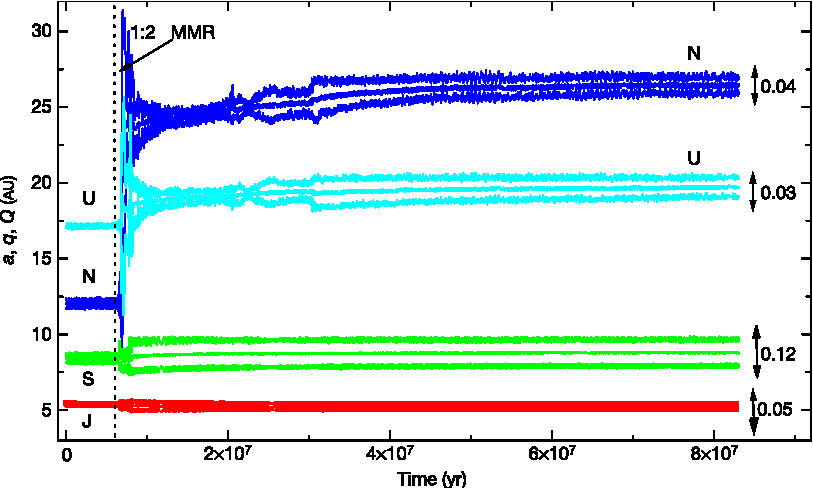
\includegraphics[scale=1]{img/Tsiganis2005-1.pdf}
\caption{Bahnveränderung der vier Gasplaneten. Über die Zeit sind die Entfernung des Perihel, die große Halbachse und Entfernung des Aphel von Jupiter (rot), Saturn (grün), Neptun (dunkelblau) und Uranus (hellblau) dargestellt. Der Zeitpunkt als es zur 1:2 MMR zwischen Jupiter und Saturn kommt ist gestrichelt eingezeichnet. Rechts sind die finalen Numerischen Exzentrizitäten angegeben. Es handelt sich hier um eine Simulation mit einer dynamisch heißen Scheibe mit $\unit[35]{\ME}$ aus 3500 Teilchen. Wie in etwa der Hälfte der Fälle kam es auch hier zu einer Vertauschung der Reihenfolge der Eisplaneten. Bild nach \cite{Tsiganis2005}.}
\label{fig:Orbitalevolution}
\end{figure}
Während der Migration werden die Exzentrizitäten durch die dynamische Reibung durch die Planetesimale, gedämpft\cite{Tsiganis2005}.
Mit der Zeit kommen die Planeten sich durch die Migration näher, so dass Mean-Motion-Resonanzen auftreten.
Man betrachtet im Nizza-Modell die 1:2-Resonanz zwischen Jupiter und Saturn, welche nach ein paar hundert Millionen Jahren auftritt.
Die Autoren testeten auch Anfangsbedingungen, welche zum Auftreten von anderen MMRs führten. Doch weder die 2:3 MMR zwischen Saturn und dem inneren Eisriesen, noch die 1:2 MMR zwischen den beiden Eisriesen waren stark genug um die Bahn von Jupiter zu beeinflussen\cite{Tsiganis2005}.
Die Resonanz führt zu einer schlagartigen Erhöhung der Exzentrizitäten der Umlaufbahnen von Jupiter und Saturn, auf Werte die mit den heutigen vergleichbar sind.
Dadurch stören Jupiter und Saturn die Eisplanenten, so dass auch deren Exzentrizitäten abhängig von den genauen Anfangsparametern (Massen und großen Halbachsen der Planeten) mehr oder weniger stark anwachsen\cite{Tsiganis2005}.
Da die Planetenorbits sehr dicht aneinander liegen, führen die hohen Exzentrizitäten zu überschneidenden Bahnen\cite{Tsiganis2005}, es kommt dadurch zu Begegnungen von Planeten.
Dies hat wiederum zwei Effekte: die Inklinationen der Planeten wächst um $1^\circ-7^\circ$ und die Eisriesen werden hinaus in die Planetesimalscheibe gestreut,
wodurch nun schlagartig eine große Menge an Planetesimalen ins Innere gestreut werden und sich folglich die Migrationsrate der Planeten drastisch erhöht\cite{Tsiganis2005}.
Die große Anzahl an kleinen Objekten im Bereich der Planetenbahnen, führt jedoch auch zu dynamischer Reibung,
wodurch die Exzentrizitäten und Inklinationen wieder langsam sinken und sich das System somit wieder stabilisiert\cite{Tsiganis2005}.
Wenn die Planetesimalscheibe fast vollständig zerstreut ist, stoppt die Migration der Planeten und sie erreichen ihre endgültigen Bahnen\cite{Tsiganis2005}.

\newcommand{\DII}{\Delta a_{\mathrm{I}_1,\mathrm{I}_2}}
\newcommand{\DSI}{\Delta a_{\mathrm{S},\mathrm{I}_1}}
Die endgültigen Bahnen hängen von dem Verhalten des Systems zum Zeitpunkt direkt nach der Resonanz ab. In den 43 Simulationen in \cite{Tsiganis2005} zeigte sich, dass von den zahlreichen Anfangsparametern der Abstand der Eisriesen $\DII$ und vor allem der Abstand zwischen Saturn und dem inneren Eisriesen $\DSI$ die größten Auswirkungen haben\cite{Tsiganis2005}.
Wie oben schon erwähnt, wurden für $\DII$ Werte zwischen etwa zwei und sechs AU verwendet, während die Werte von $\DSI$ zwischen ~2.5 und ~5 AU betrugen\cite{Tsiganis2005}.
Wählt man den Abstand zwischen Saturn und dem ersten Eisplaneten klein, so steigt die Wahrscheinlichkeit, dass einer der Eisplaneten von Saturn auf ein die Jupiterbahn kreuzendes Orbit gestreut wird und dann von Jupiter aus dem System geschleudert wird. Für $\DSI \le \unit[3]{AU} $ geschah dies in 14 der 43 Simulationen (33\%).
Wählt man den Abstand hingegen sehr groß ($\DSI \approx \unit[5]{AU}$), so ist das System möglicherweise nicht mehr kompakt genug, so dass überhaupt keine Begegnungen von Planeten stattfinden.

\begin{figure}[tbn]
\centering
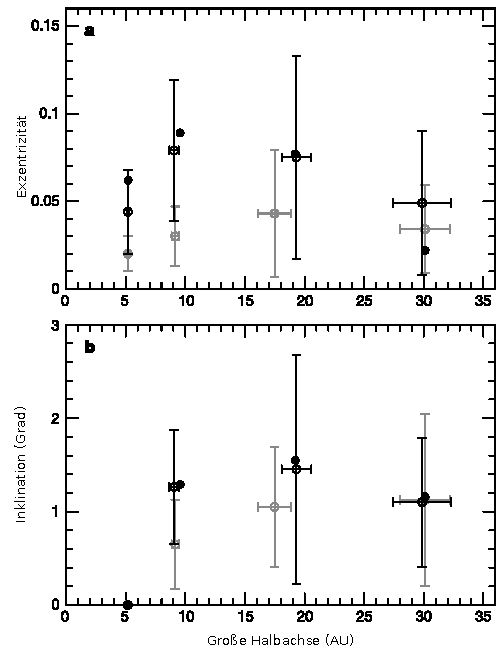
\includegraphics[scale=1]{img/Tsiganis2005-2.pdf}
\caption{Vergleich der gemittelten Simulationsergebnisse mit den tatsächlichen Messwerten der Bahneigenschaften der Gasplaneten. Aufgetragen ist \textbf{a)} die Exzentrizität beziehungsweise \textbf{b)} die Inklination über die große Halbachse. Die grauen Kreise stellen die Ergebnisse von Klasse A dar, während die schwarzen, nicht gefüllten Kreise die Messwerte für Klasse B darstellen. Die Fehlerbalken entsprechen jeweils einer Standardabweichung. Die Messwerte sind als schwarze, gefüllte Punkte eingezeichnet. Bild nach \cite{Tsiganis2005}.}
\label{fig:VergleichmitMesswerten}
\end{figure}
Für die restlichen Fälle, welche sich allesamt nach einer wie oben beschriebenen Migrationsphase wieder stabilisieren, gilt, dass es für Abstände $\DII \ge \unit[3.5]{AU}$ zwar zu Interaktionen der beiden Eisplaneten unter einander, nicht jedoch zwischen einem Eisriesen und Saturn kommt, während es in Simulationen mit kleinerem $\DII$ auch zu solchen kommt. In Übereinstimmung mit der Originalveröffentlichung, bezeichnen wir erstere Art von Simulationen als Klasse A und letztere als Klasse B\footnote{Die beiden Fälle in der es zu keiner Begegnung kam, wurden aus mir nicht ganz nachvollziehbaren Gründen nicht ausgeschlossen sondern zur Klasse A gerechnet.}, \cite{Nesvorny2007} bezeichneten Klasse A als Malhotra Klasse (MA) \citep[nach][]{Malhotra1996,Hahn1999a} und Klasse B als 'direct emplacement`-Klasse (DE).

Bei Klasse B wird Neptun durch Uranus direkt fast auf seine endgültige Entfernung geschleudert %wo, warum wichtig?
und anschließend wird die Exzentrizität durch dynamische Reibung in der Planetesimalscheibe verringert\cite{Nesvorny2007}. Somit ist die Zeitdauer der Phase der Schnellen Migration bei dieser Klasse kürzer\cite{Tsiganis2005}. Auch führt diese Art der Dynamik dazu, dass die Exzentrizität weniger stark abnimmt\cite{Tsiganis2005}.
Bei den Simulationen der Klasse A wird Neptun auf eine etwa $\unit[22-25]{AU}$ von der Sonne entfernte Umlaufbahn geschleudert und migriert dann langsamer innerhalb der Planetesimalscheibe auf seine endgültige Position\cite{Tsiganis2005}.
Die beiden Simulationsklassen, kamen etwa gleich oft vor, 14 der Simulationen waren vom Typ B, die anderen 15 waren vom Typ A.

Die Durchschnittswerte und Standardabweichungen für die großen Halbachsen, Exzentrizitäten und Inklinationen der Planeten von beiden Gruppen sind in Grafik \ref{fig:VergleichmitMesswerten} aufgetragen. Wie man sieht, stimmen die Resultate beider Klassen fast mit den tatsächlich beobachten Werten überein, im Fall der Klasse B ist die Übereinstimmung jedoch deutlich größer – hier liegen sogar alle Messwerte innerhalb nur einer Standardabweichung um den Mittelpunkt\cite{Tsiganis2005} – Klasse A hat ist etwas schlechter, insbesondere sind die Exzentrizitäten von Saturn und Uranus deutlich zu klein\cite{Tsiganis2005,Nesvorny2007}. 
Dies stellt insgesamt einen bedeutenden Erfolg des Modells dar und es hebt sich von vorhergehenden Modellen ab.
So hatte zum Beispiel das Vorgängermodell von \cite{Gomes2004} das Problem zwar vorherzusagen können, dass Neptun eine große Halbachse von etwa 30 AU hat, jedoch war die Uranusbahn dabei zu dicht an der Sonne.
Die großen Halbachsen der Eisriesen für die Klasse B betragen im Nizza-Modell hingegen $a_U = \unit[19,3 \pm 1,3]{AU}$ und $a_N = \unit[29,9 \pm 2,4]{AU}$, was mit den tatsächlichen Werten von $a_U = \unit[19,2]{AU}$ und $a_N = \unit[30,1]{AU}$ sehr gut übereinstimmt\cite{Tsiganis2005}.

Der finale Abstand zwischen Jupiter und Saturn hängt vor allem von der Masse der Materie,
die sie während der instabilen Phase streuen, ab, welche ihrerseits wiederum von der Masse der Planetenscheibe abhängt\cite{Tsiganis2005}. % richtig?
Höhere Massen der Scheibe führen zwar zu stabileren Endsystemen, wird die Masse jedoch größer als $\approx \unit[(35-40)]{\ME}$ wird der Abstand zwischen Jupiter und Saturn im fertigsimuliertem System zu groß\cite{Tsiganis2005} und wählt man eine Masse von $\approx \unit[50]{AU}$, so tritt zwischen Jupiter und Saturn zusätzlich auch eine 2:5 Resonanz auf und die dynamische Reibung wird so groß, dass Exzentrizitäten kleiner als in Realität ausfallen\cite{Tsiganis2005}.

Die dynamische Temperatur der Scheibe wirkt sich auf die Exzentrizitäten aus: Heißere Scheiben führen zu höheren Exzentrizitäten von Jupiter und Saturn. Die beobachtete Existenz von zahlreichen plutogroßen transneptunischen Objekten spricht laut den Autoren für eine Scheibe mit der Dynamik der heißeren der beiden getesteten Scheiben\cite{Stern1991,Tsiganis2005}.

\begin{figure}[tbn]
\centering
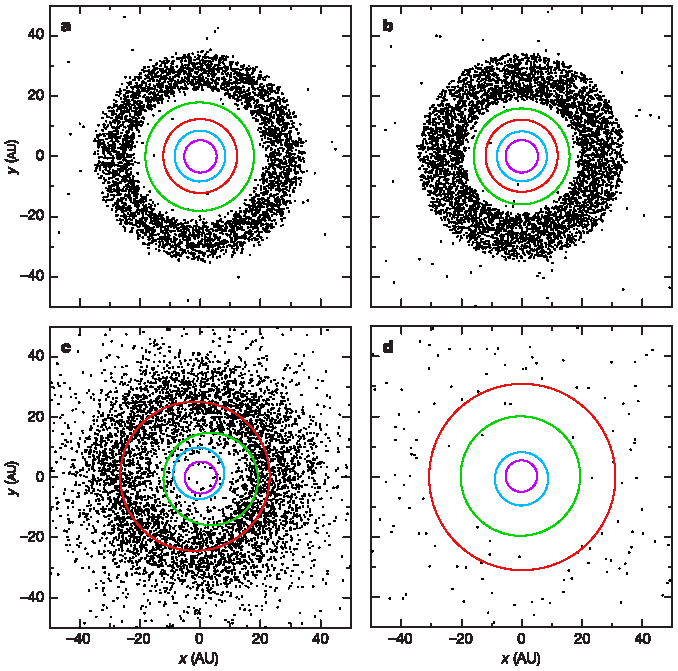
\includegraphics[scale=1]{img/Gomes2005-2.pdf}
\caption{Die Planetenorbits und die Positionen der Teilchen während einer Simulation. Projektion auf die mittlere Orbitalebene. Abbildung \textbf{a)} zeigt das System nach nur 100 My zum Beginn der Migration. Abbildung \textbf{b)} stellt das System kurz vor dem Auftreten des Resonanzfalls dar (879 My). Abbildung \textbf{c)} zeigt das System nur 3 Millionen Jahre nach \textbf{b)} dar. Abbildung \textbf{d)} zeigt das System weitere 200 Millionen Jahre später, nur noch wenige Planetesimale sind übrig. Bild nach \cite{Gomes2005}.}
\label{fig:Zeitlicheentwicklung}
\end{figure}

\FloatBarrier
\section{Late Heavy Bombardment}\label{LHB}
Geologische Untersuchungen von Mondgestein zeigten, dass es vor 3,9-4,0 Milliarden Jahren -- also 700 Millionen Jahre nach der Plantenentstehung --
eine enorme Häufung von Einschlägen gab.\footnote{Neuere Untersuchungen von \cite{Bottke2012} datieren das LHB auf 4,1-4,2 Milliarden Jahre vor heute. Wie in diesem Kapitel ersichtlich werden wird, beeinträchtigt dies das Nizza-Modell nicht. Aus Gründen der Konsistenz werde ich daher den zur Zeit von \cite{Gomes2005} aktuellen Wert verwenden.} Man nennt dieses Ereignis das Late Heavy Bombardment (LHB) oder auf deutsch auch das Große Bombardement\cite{Tera1974,Hartmann2000,Ryder2002}.
Die Planetenentstehungsmodelle können eine solche Häufung zu einem so spätem Zeitpunkt nicht erklären.
Es gab bereits zuvor einige Modelle zur Erklärung des LHBs \citep[insb.][]{Zappal1998Icar,Levison2001Icar,Chambers2002LPI,Levison2004ASPC} jedoch waren diese relativ gekünstelt und kein notwendiger Bestandteil der ansonsten abgeschlossenen Beschreibung der Entwicklung des Sonnensystems\cite{Gomes2005}.
Im Rahmen des Nizza-Modells liegt es natürlich nahe anzunehmen das LHB sei durch die während der Instabilitätsphase zerstreuten Objekte der Planetesimalenscheibe entstanden.

Da die Planetesimalenscheibe aufgrund ihrer sonnenfernen Entstehung vermutlich eisig war und sie, wie wir in Kapitel \ref{Kuiper} sehen werden, der Ursprung der heutigen transneptunischen Objekte war, kann man sie im folgenden getrost als Kometen bezeichnen\cite{Gomes2005}. % wohin damit?

\begin{figure}[tbn]
\centering
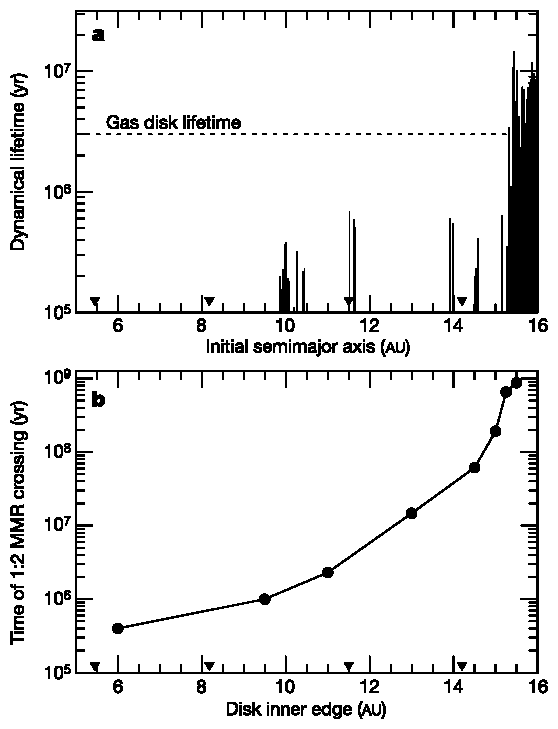
\includegraphics[scale=1]{img/Gomes2005-1.pdf}
\caption{\textbf{a)} Um zu ermitteln ob und wo die Planetesimalenscheibe für die Anfangsbedingung des Nizza-Modells existiert, haben \cite{Gomes2005} in einer eigenen Simulation die dynamische Lebenszeit von Planetesimalen im frühen Sonnnensystem ermittelt. Die Planeten wurden dabei auf nahezu kreisförmigen, planaren Orbits mit großer Halbachse von 5,45, 8,18, 11,5 und $\unit[14,2]{AU}$ (schwarze Dreiecke) gesetzt. Für unterschiedliche Entfernungen wurden jeweils 10 Teilchen auf Orbits mit $e=i=0$ gesetzt, die mittlere Lebensdauer von 10 solchen Teilchen ist jeweils als Strich eingezeichnet. Ein Vergleich mit der Lebensdauer der Gasscheibe bestätigt die Anfangsbedingungen des Nizza-Modells und zeigt, dass der innere Rand der Gasscheibe etwa $\unit[1-1,5]{AU}$ hinter dem zweiten Eisriesen sein musste.
\textbf{b)} Zeit nach welcher es zu der Resonanz zwischen Jupiter und Saturn kommt, in Abhängigkeit von der Position des inneren Randes der Planetesimalenscheibe. Die Dichte und Gesamtmasse der Scheibe wurde dabei konstant gewählt. Man sieht, dass für die in {\textbf{a)}} ermittelten plausiblen Werte die Ressonanz erst nach etwa $\sim10^9$ Jahren eintritt, was gut zum Zeitpunkt des LHB passt. Bild nach \cite{Gomes2005}.}
\label{fig:LHBtiming}
\end{figure} % Aufteilen in zwei Grafiken? oder umwandeln in Queerformat
\begin{figure}
\centering 
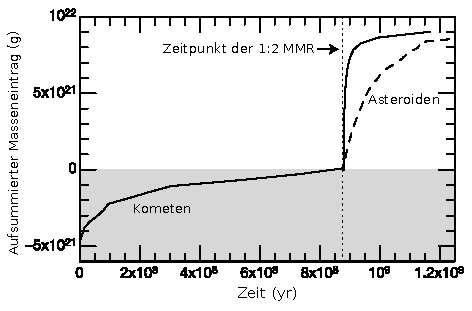
\includegraphics[scale=1]{img/Gomes2005-3}
\caption{Durch Kometen und Asteroideneinschläge auf dem Mond eingebrachte Gesamtmasse in Abhängigkeit von der Zeit. Die Y-Achse wurde so Verschoben, dass sie zum Zeitpunkt der Resonanz (gestrichelt) den Wert Null hat, so ist ersichtlich, dass unmittelbar nach dem Überschreiten der MMR innerhalb kurzer Zeit etwa $\unit[9\cdot10^21]{g}$ Masse durch Kometen eingetragen wird. Bild nach \cite{Gomes2005}.}
\label{fig:LHBMasse}
\end{figure}
Vorgängermodelle des Nizza-Modells hatten das Problem, dass die schnelle, durch das Streuen von Planetesimalen bedingte, Migration unmittelbar nach Simulationsbeginn eintrat und man somit nicht erklären konnte warum das LHB erst nach etwa 700 Myr stattfand.
Dies lag jedoch an einer falschen Startbedingung: Man hatte hierbei die Planetesimalen in direkte Umgebung zu den Planeten gesetzt, was zwar zu einer gewünschten Migration führt, jedoch eine unnatürliche Startsituation ist,
denn es ist davon auszugehen, das die Migration durch Interaktion mit den Planetesimalen zum Zeitpunkt als das System noch in der Gasscheibe eingebettet war, im Vergleich zur Migration durch Interaktion mit der Gasscheibe vernachlässigbar ist.
Deshalb sollte die Anfangsbedingung des Nizza-Modells gerade den Zustand darstellen, in welchem sich das Sonnensystem direkt nach dem Auflösen der Gasscheibe befand. Betrachten wir also diesen Zeitpunkt, so sollten alle existierenden Planetesimale sich auf Orbits befinden, die stabil genug sind um bis zu diesem Zeitpunkt überhaupt überlebt zu haben.
Die Planetesimalscheibe sollte also nur Teilchen auf Bahnen haben deren dynamische Lebenszeit größer als die Lebensdauer der Gasscheibe – typischerweise $\unit[3-10]{Myr}$\cite{Haisch2001} – ist\cite{Gomes2005}.
Berücksichtigt man diese Bedingung, erhält man die schon in Kapitel \ref{Orbits} vorgegriffene Anfangsbedingung, das die Planetesimalscheibe hinter dem letzten Planeten beginnt, und zwar hinter etwa 15,3 AU\cite{Gomes2005}.

Die anfängliche Migrationsrate hängt nun von der Rate ab, mit welcher Planetesimale auf Planetenorbits schneidende Orbits gestreut werden. Die Zeitdauer bis zum Auftreten der MMR hängt schließlich von den folgenden Parametern ab:
1. Dem Anfangsabstand zur Ressonanz, 2. der Dichte der Scheibe am inneren Rand und 3. der Abstand zwischen dem inneren Rand der Scheibe und dem äußeren Eisplaneten\cite{Gomes2005}.

In acht Simulationen untersuchten \cite{Gomes2005} die Abhängigkeit des Ressonanzzeitpunktes in Abhängigkeit von der Position des inneren Rands der Planetesimalscheibe, bei ansonsten gleichen Parametern – inklusive gleicher Scheibenmasse und Dichte. Wie in Bild \ref{fig:LHBtiming} zu sehen ist, steigt die Zeit stark mit der Entfernung des inneren Rands an. Für große Werte $\gtrsim \unit[15,3]{AU}$ wie wir sie oben erhalten haben, tritt die Resonanz 192 bis 880 Millionen Jahre nach Beginn der Simulation auf, was zum Zeitpunkt des LHB passen würde. % Achtung: nach beginn der Simulation, nicht nach Planetenentstehung wie oben.
Durch zusätzliche Variation anderer Parameter konnte das Eintreten der Resonanz auf bis zu 1,1 Milliarden Jahre\cite{Gomes2005} verzögert werden – somit ist klar, dass das späte Auftreten des großen Bombardements bei geeigneter Parameterwahl durchaus leicht erklärt werden kann.

Als zweite wichtige Überprüfung, untersuchten die Wissenschaftler die Masse des auf den Mond treffenden Materials an. Bei den Simulationen waren dies etwa $\unit[9 \cdot 10^{21}]{g}$, davon trafen 50\% den Mond in den ersten 3,7 Millionen Jahren, 90\% in den ersten 29 Millionen Jahren. Das Bombardement fand demnach während einer relativ kurzen Zeitspanne statt. Die dabei durchschnittlich auf dem Mond treffende Gesamtmasse wurde auf $\unit[\left(8,4 \pm 0,3\right) \cdot 10^{21}]{g}$ bestimmt\cite{Gomes2005}.

Hinzu kommt, dass es bei der Migration von Jupiter und Saturn von ihrer Position in der 1:2-MMR zu ihren heutigen Orbits zu einer säkularen Resonanz kommt, welche über den Asteroidengürtel streifen.
Durch diese können Asteroiden Orbits mit so großen Exzentrizitäten und Inklinationen erhalten, so das diese bis ins innere Sonnensystem reichen. Wir müssen also die Masse der Asteroiden bestimmen, welche zusätzlich zu den Planetesimalen mit dem Mond kollidieren.
Dafür führten die Autoren weitere numerische Simulationen durch, in welchen sie die Auswirkungen von Sonne, Venus, Erde, Mars, Jupiter und Saturn auf den aus 1.000 masselosen Teilchen modellierten Asteroidengürtel untersuchten.
Die Migration der Gasriesen wurde dabei, durch das Hinzufügen von geeigneten Termen zur Bewegungsgleichung, künstlich erzwungen.
Die großen Halbachsen der Asteroiden betrugen dabei zwischen $\unit[2]{AU}$ und $\unit[3,5]{AU}$ und hatten Exzentrizitäten zwischen 0 und 0,3, sowie Inklinationen zwischen 0\degree und 30\degree – wobei das Perihel immer größer als $\unit[1,8]{AU}$ und das Aphel immer kleiner als $\unit[4]{AU}$ gewählt wurde.
Diese Orbitalverteilung entspricht in etwas heutigen, was gerechtfertigt ist, da die Entstehungsmodelle des Asteroidengürtels davon ausgehen, dass dieser schon vor dem LHB seine heutige Orbitalverteilung erhielt\cite{Wetherill1992,Petit2001,Gomes2005}.
Als Migrationsraten wurden in den Simulationen unterschiedliche Resultate der ursprünglichen Simulationen (\refsec{Orbits}) gewählt.

\cite{Gomes2005} unterscheiden zwei Wege, auf welchen ein Asteroid auf ein die Erdbahn kreuzendes Orbit kommen kann: (1) Entweder es kommt zu einer säkularen Resonanz zwischen der Periheldrehung des Körpers und der Periheldrehung Saturns, wodurch die Exzentrizitäten des Asteroiden steigen und er auf eine erdbahnkreuzende Bahn gelangt, oder (2) sie werden im Asteroidengürtel dynamisch angeregt und wandern dann langsam aus dem Asteroidengürtel heraus.
Weg (1) ist schneller, so das 50\% der Einschläge dieser Art bereits in den ersten 10 Myr (90\% in 30 Myr) stattfinden, während die Einschläge durch, auf letztere Art auf Kollisionskurs gebrachte, Asteroiden innerhalb von 50 Myr zu 50\% stattfanden (90\% in 150 Myr)\cite{Gomes2005}.
In den Simulationen von \cite{Gomes2005} war der zweite Typ häufiger, wobei dies wenig aussagt, da
die Häufigkeitsverteilung der beiden Wege vermutlich stark von den genauen Migrationsraten und den genauen dynamischen Zustand des Asteroidengürtels abhängt.
Die Masse an Asteroiden die den Mond gemäß diesen Simulationen trifft wurde auf $\unit[\left( 3-8 \right) \cdot 10^{21}]{g}$, % anderer strich statt minus? space
also einen ähnlich hohen Wert wie für die Planetesimale bestimmt – wobei die Unsicherheiten bei der Bestimmung der Masse der Asteroiden zu groß ist um ein Verhältnis zwischen den beiden Komponenten anzugeben. Auch ist noch nicht genau untersucht worden, inwieweit dieses Verhältnis eine Funktion von der Zeit und der Teilchengröße ist – so waren in diesen Simulationen die Planetesimale in den ersten 30 Millionen Jahren dominierend, während die Asteroiden länger auf den Mond niederprasselten\cite{Gomes2005}.

Die Dauer des LHB beträgt in diesem Modell zusammenfassend also zwischen 10 und 150 Millionen Jahren – eine genauere Bestimmung ist nicht möglich. Dafür würde man sowohl das Verhältnis zwischen den Anteilen der beiden Asteroiden streuenden Mechanismen, sowie das Verhältnis dieser zu dem Anteil an Planetesmialen kennen. Und da diese sehr sensibel von den genauen Anfangsparametern – insbesondere der genauen anfänglichen Struktur des Asteroidengültels – abhängen, konnten sie nicht bestimmt werden\cite{Gomes2005}.

Vergleichen wir nun die Vorhersagen des Modells mit bekannten Messgrößen. Das Nizza-Modell kann den für andere Modelle problematischen späten Zeitpunkt des Bombardements erklären. Auch die Menge des dabei auf den Mond eingebrachten Materials passt größenordnungsmäßig gut: So wurde aus der Anzahl und Größe der Mondkrater eine ungefähre Masse von $\unit[6 \cdot 10^{21}]{g}$ bestimmt\cite{Levison2001b,Gomes2005}, während die Simulationen $\unit[\left(8,4 \pm 0,3\right) \cdot 10^{21}]{g}$ an Planetesimalen und weitere $\unit[\left( 3-8 \right) \cdot 10^{21}]{g}$ an Asteroiden ergab.
Das Modell sagt wie schön in Bild \ref{fig:LHBMasse} zu sehen einen sehr plötzlichen Beginn des Bombardements voraus. Leider sind die bisher Beobachtungsdaten noch zu schlecht um dies zu überprüfen.
Das Nizza-Modell sagt voraus, dass sowohl Asteroiden, also auch Planetesimale auf dem Mond eingeschlagen sind, dies stimmt damit überein, dass kosmochemische Analysen davon ausgehen, dass einige der Mondkrater durch Einschläge von Asteroiden geformt wurden.
Die Streuung von Asteroiden führt auch dazu, dass der Asteroidengürtel um einen Faktor von ungefähr 10 ausgedünnt wird. Dies passt zu bestehenden Modellen, welche die fortlaufende Entwicklung des Asteroidengürtels durch Kollisionen beschreiben und erklärt warum es keine großen Asteroidenfamilien gibt, die zur Zeit des LHB entstanden sind\cite{Davis1994,Bottke2005,Gomes2005}.
Die Menge an Kometen, die während des LHB auf die Erde trafen ergibt sich im Nizza-Modell zu $\approx \unit[1,8 \cdot 10^{23}]{g}$ was etwa 6\% der heutigen Ozeanmasse beträgt und somit kompatibel zu der durch Isotopenhäufigkeit (D-zu-H-Verhältnis) bestimmten Obergrenze der durch Kometen eingebrachten Wassermenge ist\cite{Morbidelli2000,Gomes2005}.

Abschließend möchte ich noch darauf hinweisen, dass die Existenz des Late Heavy Bombardments nicht ganz unumstritten ist. Zuletzt hat insbesondere die geologische Untersuchung von \cite{Spudis2011} die Notwendigkeit der Existenz in Frage gestellt. Die Autoren des Nizza-Modells gehen darauf unter anderem auch in \cite{Brasser2009} darauf ein. Sie führen auf, dass es vier verschieden Gründe gibt, die für das LHB sprechen:
\begin{enumerate}
\item Die Existenz besonders große Mare wie Imbrium und Orientale auf dem Mond ist nicht mit einer monoton abfallender Einschlagsrate -- wie von Modellen ohne Migration der Riesenplaneten vorhergesagt -- erklärbar \cite{Bottke2007}
\item Untersuchungen von Zirkonen, deuten darauf hin, dass das Erdklima vor 4,3-3,9 Milliarden Jahren vergleichsweise kalt und vor 3,8 Milliarden Jahren -- vermutlich durch die Einschläge während des LHBs -- deutlich erwärmt wurde\cite{Mojzsis2001,Trail2007}
\item die größten Mare des Monds entstanden erst nach dem Zusammenbruch des Marsianischem Magnetfeld \cite{Lillis2006,Lillis2007}
\item der Saturnmond Iapetus weist Einschlagskrater auf die jünger sind, als der der vor 200 bis 800 Millionen Jahren entstandene Äquatoriale Bergrücken\cite{Castillo-Rogez2007}
\end{enumerate}

\FloatBarrier
\section{Trojaner}\label{Trojaner}
\newcommand{\PJS}{P_J/P_S}

\begin{figure}
\centering 
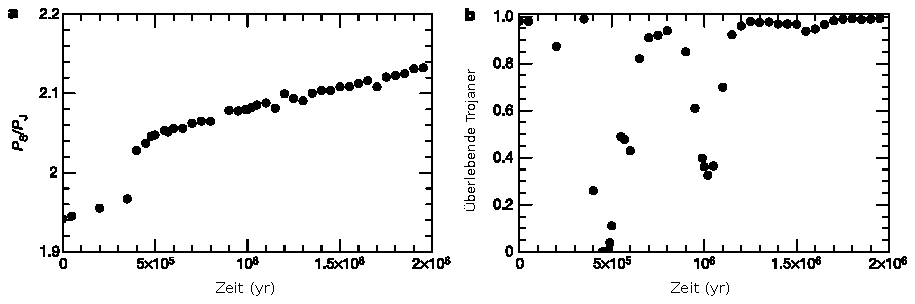
\includegraphics[scale=1]{img/Morbidelli2005-1v}
\caption{Stabilität der Trojaner während der Migrationsphase. \textbf{a)} zeigt das aus den Simulationen entnommene Verhältnis der Umlaufdauer von $\PJS$, der Sprung entspricht der Überquerung der 1:2 MMR. In \textbf{b)} wurden anschließend für diese Messwerte ermittelt, wie viele Trojaner über $2\cdot10^5$ Jahre überleben. Bild nach \cite{Morbidelli2005}.}
\label{fig:Trojanerstabilitaet}
\end{figure}
\begin{figure}
\centering 
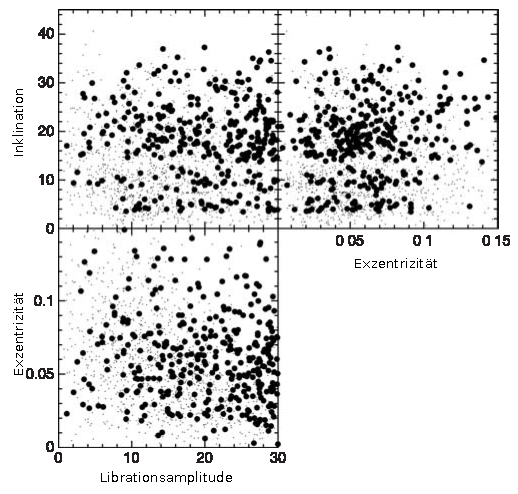
\includegraphics[scale=1]{img/Morbidelli2005-2}
\caption{Vergleich der Orbits der Trojaner in der Simulation (dicke schwarze Punkte) mit den Messwerten (graue Punkte). Bild nach \cite{Morbidelli2005}.}
\label{fig:Trojanerorbitale}
\end{figure}
Als Trojaner bezeichnet man Objekte, die auf dem selben Orbit wie ein Planet kreisen, jedoch um 60\degree\ vor- oder rückläufig, um die Lagrange-Punkte L4 und L5 des Planeten. 
Man kennt bereits über 6.000 Trojaner in des Lagrange-Punkten Jupiter, daneben kennt man auch 9 Trojaner von Neptun und 4 Mars- und je einen Uranus- und Erdtrojaner\cite{IAU14}.
Da die terrestrischen Planeten beim Nizza-Modell weitgehend ignoriert werden, sind auch die Trojaner von Mars und Erde für diese Arbeit nicht von Belang.

Die Jupiter-Trojaner wurden in der Literatur häufig als Argument gegen das Auftreten der 1:2-MMR zwischen Jupiter und Saturn genannt. Das Überschreiten der Resonanz würde die Trojanerbahnen destabilisieren und die Trojanerpopulation vollständig auslöschen\cite{Gomes1998,Michtchenko2001,Morbidelli2005}.
Mit einer Simulation durch \cite{Morbidelli2005} zeigt sich dies ebenfalls: kein einziger der Trojaner überlebte das Überschreiten der Resonanz.

Man ging bisher davon aus, dass die Trojaner sich in der Nähe von Jupiter gebildet haben und, als Jupiter wuchs, entweder durch Kollisionen oder durch Reibung mit Gas eingefangen wurden\cite{Yoder1979Icar,Shoemaker1989aste,Peale1993Icar,Kary1995Icar,Marzari1998Icar,Fleming2000Icar,Kortenkamp2001DPS,Morbidelli2005}. 
Diese Theorie hat jedoch das Problem, dass es unter anderem die große Inklinationsverteilung der Trojaner von bis zu 40\degree\ nicht erklären kann\cite{Marzari2002,Morbidelli2005}.
Da die Entwicklung von gravitativen Systemen zeitreversibel ist, können auf den selben Bahnen,
auf welchen die Trojaner von ihren Co-Orbitalen Bahnen entkommen können, auch Objekte vorübergehend auf Trojanerbahnen gelangen.
Somit ergibt sich im Rahmen des Nizza-Modells ein alternatives Entstehungsmodell der Trojanerpopulationen: Während der Insablilitätsphase direkt nach Überquerung der Resonanz sind die Co-Orbitalbahnen um die Lagrangepunkte dynamisch offen, so, dass eventuell vorhandene Trojaner entweichen können, genauso können jedoch die zahlreichen Planetesimale, die im Nizza-Modell für die Migration verantwortlich sind, durch diese Gebiete wandern.
Sobald sich die Jupiter- und Saturnbahnen weit genug von der Resonanz entfernt haben, wird die Region wieder stabil und die Objekte die zu diesem Zeitpunkt dort sind, sind von nun an dort gefangen und bilden die heute beobachtbaren Jupiter-Trojaner.

Um dieses Konzept zu prüfen, untersuchten \cite{Morbidelli2005} zunächst wann genau es zum Verlust der Trojaner kommt, also wann die Co-Orbitalregionen offen sind.
Dazu führten Sie eine zweistufige Simulation durch. Im ersten Stritt wählten sie eine der ursprünglichen Simulationen, wobei sie – aus Gründen, die später ersichtlich werden, – eine Simulation mit relativ langsamer Migration wählten. %wird es von alleine offensichtlich?
In dieser Simulation maßen sie zu 40 Zeitpunkten das Verhältnis $\PJS$.
Nun simulierten sie für jeden dieser Werte das System, um zu messen wie viele der Trojaner verloren gehen. Diese Simulationen umfassten jeweils die Sonne, Jupiter und Saturn (bei festem Verhältnis von $P_J/P_S$) sowie eine große Anzahl an masselosen Testteilchen und liefen über $\unit[2\cdot10^5]{yr}$.
Abbildung \ref{fig:Trojanerstabilitaet} zeigt die Messwerte von $\PJS$ und den Anteil an Körpern welche den Simulationszeitraum überlebten. Man sieht zwei deutliche Minima, welche auch theoretisch erklärt werden können.
Bei $\PJS \approx 2.05$ tritt eine sekundäre 3:1 Resonanz zwischen $1/P_J-2/P_S$ und der Oszilationsfrequenz mit der die Trojaner um den Lagrangepunkt kreisen auf, diese führt zu einer vollständigen Destabilisierung der Gebietes und somit zum Verlust aller Trojaner.
Ein zweites Minimum ergibt sich durch die 1:2 Resonanz selbiger Größen und führt zum Verlust von etwa 70 \% der Trojaner.
Gemäß dem Zeitreversibilitätsprinzip sind dies auch die Zeiten, bei welchen ein Einfang von Planetesimalen wahrscheinlich ist.

Um nun die Theorie zu testen, führten sie zwei Simulationen durch,
wobei der als ''langsame Simulation`` bezeichnete Durchlauf die Geschwindigkeit von oben verwendet, während die ''schnelle Simulation`` eine drei mal schnellere Migration vorwies – somit stellen diese die langsamsten und schnellsten Migrationsfälle des Nizza-Modells dar. Da dies für die Betrachtung der einzige wichtige Parameter ist, ist der Parameterraum abgedeckt.
Für den Zeitraum zwischen dem Beginn der ersten sekundär-Resonanz und dem Ende der zweiten, wurde ein konstanter Strom von Planetesimalen durch das System geschickt,
zeitgleich wurden die Planeten durch Hinzufügen von geeigneten Krafttermen in die Bewegungsgleichungen zur Migration gezwungen.
Die Testteilchen wurden dafür auf, die Saturnbahn kreuzende Orbits, mit Exzentrizitäten und Inklinationen wie in den ursprünglichen Simulationen beobachtet, gesetzt und immer wenn ein Teilchen aus dem System verloren ging wurde es wieder auf sein ursprüngliches Orbit gesetzt, so das die Teilchenanzahl immer konstant 1.163.000 betrug.
Insgesamt wurden in der langsamen Simulation 5.466.000 Teilchen entfernt und wieder eingefügt, 98 Teilchen endeten nach $1,2 \cdot 10^6$ Jahren – als sich die Co-Orbitalregionen stabilisiert haben – auf Trojanerbahnen.
Die wurden 19 mal kopiert %erklären wohin
 und dann über weitere 10 Myr simuliert um ihre langzeitliche Stabilität zu testen.
Dabei wurden die Exzentrizitäten der Planeten durch Zusatzterme in den Bewegungsgleichungen, wie im Nizza-Modell beobachtet, gedämpft. Am Ende überlebten 266 Teilchen. Die gesamte Eingangseffizienz berechnet sich als $266/20/5466000 \approx 2,4 \cdot 10^{-6}$.
Bei der schnellen Migration wurde die Migrationsgeschwindigkeit verdreifacht und die Simulationszeit entsprechend gedrittelt, ansonsten blieb sie unverändert.
Bei dieser wurden insgesamt 2.773.000 Teilchen entfernt und wieder eingefügt und 174 Teilchen endeten auf Trojanerorbits. Sie wurden 9-mal geklont, 486 Teilchen überlebten am Ende.
Die Effizienz beträgt somit $486/10/2773000 \approx 1,8 \cdot 10^{-5}$.
In beiden Simulationen hatten etwa die Hälfte der der Trojaner Librationsamplituden $D$ von weniger als 30\degree\ – wie etwa 87\% der bekannten Trojaner.
Da viele der Trojaner mit größeren Librationsamplituden auf sehr großen Zeitskalen instabil sind, passt dies mit der Beobachtung überein und für die weiteren Analysen wurden nur die Trojaner mit $D<30^\circ$ betrachtet. % Librationsamplitude erklären
Um zu überprüfen, ob die Vernachlässigung von Uranus und Neptun gerechtfertigt war,
wurden einige der Simulationen unter Berücksichtigung der Effekte dieser wiederholt, dabei stellten
\cite{Morbidelli2005} fest, dass die Eisgiganten keinen Einfluss auf die Trojaner von Jupiter haben, es ist also möglich sie zu ignorieren um Rechenzeit zu sparen.

Aus den ursprünglichen Simulationen des Nizza-Modells,
wurde die Masse der Planetesimale, die während der Instabilitätsphase durch das Sonnensystem streifen, auf $\sim \unit[3,4]{\ME}$ bestimmt.
Die Masse der Trojaner mit Librationsamplitude von unter 30\degree berechnet sich als Produkt dieser Masse mit der Einfangseffizienz und einem Faktor $1/2$, da nur die Hälfte eine Librationsamplitude von $<30^\circ$ haben. Sie beträgt für die langsame Simulation $\sim\unit[4\cdot 10^{-6}]{\ME}$ und für die schnelle Simulation $\sim \unit[3\cdot 10^{-5}]{\ME}$.
Als Theoretische Begründung für das starke Anwachsen der Masse mit steigender Migrationsgeschwindigkeit nennen die Autoren eine Kombination von zwei Gründen:
zum einen ist durch die schnellere und somit kürzere Migration bei gleicher Gesamt\/teilchenzahl die Teilchenstromdichte während der Instabilitätsphase um den selben Faktor 3 höher, wodurch auch dreimal so viele Objekte eingefangen werden. Zum anderen führt eine schnellere Migration auch zu einem schnellerem Übergang vom instabilen zum stabilen Zustand, wodurch die Einfangquote steigt\cite{Morbidelli2005}.
Beim Vergleich mit dem Literaturwert von \cite{Jewitt2000} stellen \cite{Morbidelli2005} eine deutlich Differenz fest: der berechnete Wert ist um einen Faktor $\sim 3-25$ kleiner als der Literaturwert.
Allerdings – so argumentieren die Autoren – beruhte die Berechnung von Jewitt und Kollegen auf inzwischen veralteten Messwerten zu den Trojanerpopulationen. % Auflisten?
Nach Korrektur dieser erhielt die Gruppe um Morbidelli eine Masse von $\unit[1,3 \cdot 10^{-5}]{\ME}$ für die Trojaner. Nachdem 87\% der Trojaner eine Librationsamplitude von unter 30\degree haben, ergibt sich für diese eine Masse von etwa $\unit[1,1 \cdot 10^{-5}]{\ME}$, was mit den Werten der Simulationen gut übereinstimmt\cite{Morbidelli2005}.

Als nächstes analysierte die Gruppe um Morbidelli die Orbits der eingefangenen Objekte. Dazu simulierten sie die Entwicklung der Trojaner bei abgeschlossener Migration unter Einfluss von nur der Sonne und Jupiter für weitere $10^5$ Jahre und filterten die kurzzeitigen Oszillationen der Orbits heraus.
Die Verteilung der Orbitaleigenschaften der Trojaner wiesen zwischen den beiden Simulationen keine signifikanten Unterscheide auf, weshalb sie zur Verbesserung der Statistik gemeinsam betrachtet wurden.
Grafik \ref{fig:Trojanerorbitale} zeigt die Bahneigenschaften der Simulationsergebnisse im Vergleich zu den gemessenen, wie man sieht gibt es eine gute Übereinstimmung, alle beobachteten Jupitertrojaner könnten also durch dieses Modell erklärt werden.
Das gilt auch für Objekte mit $D<5^\circ$, welche in früheren Modellen am schwersten erklärt werden konnten\cite{Marzari2002,Morbidelli2005},
und für den gesamten Bereich der Inklinationen der, wie oben schon erwähnt, bisher nicht erklärt werden konnte.

Ein weiterer positiver Aspekt an diesem Model ist, dass er erklärt warum die Jupiter-Trojaner nur sehr wenig Wasser und organische Stoffe enthalten\cite{Emery2004}:
Bevor sie als Trojaner eingefangen wurden, durchgingen sie eine Phase mit sehr hohen Exzentrizitäten, in welcher sie der Sonne immer wieder sehr nahe kamen und dabei entgasten.
Alle Trojaner der Simulation waren für mindestens 100 Jahre auf Orbits mit einem Perihel $q\lesssim \unit[3]{AU}$, 72\% der Teilchen waren mit 10.000 Jahren lange genug auf derartigen Bahnen um vollständig zu entgasen\cite{Levison1997,Morbidelli2005}.

In den ursprünglichen Simulationen von \cite{Tsiganis2005} wurde auch der Einfang einiger Neptun-Trojaner beobachtet. Durchschnittlich wurden pro Simulation zwei semistabiele (Lebenszeit $>\unit[80]{Myr}$) Trojaner eingefangen, was einer hohen Einfangeffizienz entsprechen würde\cite{Tsiganis2005}.
Die Neptun-Trojaner wurden nach einiger Zeit wieder aus ihren Orbits geworfen, was jedoch möglicherweise nur ein Artefakt der Simulation war\cite{Tsiganis2005}. % graininess of Neptuns migration
Eine genauere Analyse steht aus. % Oder ich hab sie nur noch nicht gelesen!

\FloatBarrier
\section{Die Monde der Riesenplaneten}\label{Monde}
Eine weitere wichtige Frage bei der Beschäftigung mit dem Nizza-Modell ist ob dieses Modell mit der Existenz der Monde der Gasriesen konsistent ist.
Wie wir sehen werden, ist dies in weiten Bereichen der Fall, auf Grundlage des Nizza-Modells wurde insbesondere ein neuer Entstehungsmechnismus für viele der Monde vorgeschlagen, welcher einige Vorteile gegenüber bisherigen Theorien hat. Zunächst will ich jedoch den Begriff der Hill-Sphäre einführen.

Als Hill-Sphäre bezeichnet man das in erster Näherung kugelförmige Gebiet um einen Körper (in der Regel ein Planet) der einen zweiten (hier die Sonne) umkreist, in welchem die Gravitationskräfte des Planeten überwiegen. Dabei entspricht der Radius der Hill-Sphäre der Entfernung bis zum ersten beziehungsweise zweiten Lagrange-Punkt und berechnet sich zu\cite{Sheppard2005}:
\begin{equation} 
r \approx a \sqrt[3]{\frac{m}{3 M}}
\end{equation} % die Wurzel ist häßlich
Monde können nur in einer Stabilitätszone innerhalb der Hillsphäre existieren, deren Größe von der Umlaufrichtung des Trabanten abhängt. Für Monde auf prograden Bahnen, also solche, die dieselbe Umlaufrichtung haben, in der auch der Planet um die Sonne kreist, reicht die Stabilitätszone bis zu eine Entfernung von 53\% des Hill-Radius.
Für retrogarde Trabanten reicht die Stabilitätszone hingegen bis 69\% des Hill-Radius hinaus\cite{Hamilton1997}.

Im folgenden wird zwischen zwei grundsätzlich verschiedenen Gruppen von Monden unterschieden.
Reguläre Monde findet man sehr nahe um den Planeten (bis zu $0.05 \, r_\mathrm{H}$) auf Orbits mit sehr niedrigen Exzentrizitäten und Inklinationen und ausnahmslos immer auf prograden Bahnen\cite{Sheppard2005}.
Als irregulären Mond bezeichnet man hingegen einen natürlichen Satelliten auf Orbits die weit vom Planeten entfernt sind und eine starke Inklination haben\cite{Nesvorny2007}.
Häufig haben Sie auch retrograde Umlaufbahnen und große Exzentrizitäten\cite{Nesvorny2007}.

\subsection{Reguläre Monde}
Während der Instabiliätsphase kommen sich die Planeten Saturn, Uranus und Neptun immer wieder sehr nahe, derartige Planetenbegegnungen könnten die Bahnen von Monden destabilisieren und sie aus ihrer Umlaufbahn um den Planeten werfen oder aber zumindest ihre Exzentrizitäten und Inklinationen soweit erhöhen, dass sie im Widerspruch zu den Beobachtungen liegen.
Um dies für reguläre Monde zu testen, zeichneten \cite{Tsiganis2005} bei acht ihrer Simulationen alle Begegnungen von Planeten, bei welche sich die Planeten näher als ein Hill-Radius kamen, auf.
Anschließend simulierten sie die Mondsysteme der Planeten unter dem Einfluss der Begegnungen.
Als Mondsystem verwendeten sie für Saturn dessen heute bekannten Monde und für die beiden Eisgiganten die heute bekannten Monde von Uranus\cite{Tsiganis2005}.
In der Hälfte der Simulationen überlebten nach allen Begegnungen alle Monde auf Bahnen mit $\sin i, e < 0.05$, weshalb die Gruppe um Tsiganis schloss, dass die Existenz der regulären Monde nicht im Widerspruch zum Nizza-Modell steht\cite{Tsiganis2005}.
Dies gilt jedoch nur für die regulären Monde, die irregulären Monde sind hingegen wesentlich schwächer gebunden und würden die Begegnungen deshalb nicht überleben.

\subsection{Irreguläre Monde}

\begin{figure}[tbn]
\centering
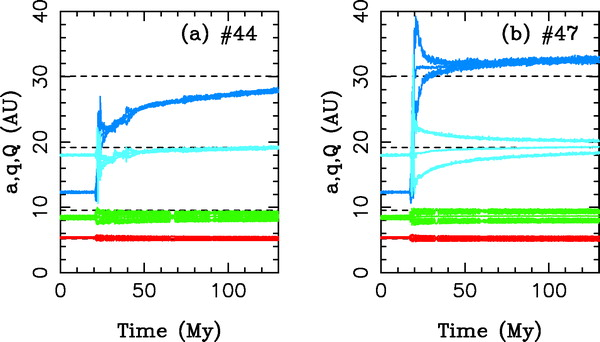
\includegraphics[scale=0.9]{img/Nesvorny2007-1}
\caption{Vergleich der Migration bei einer Simulation von Klasse A (\textbf{a)}) und Klasse B (\textbf{b)}), analog zu Abbildung \ref{fig:Orbitalevolution}. Gestrichelt sind die heutigen Positionen von Saturn, Uranus und Neptun eingezeichnet. Während bei der Klasse A die Eisriesen nach der Chaotischen Phase auf ihre heutigen Positionen migrieren, werden sie bei Klasse B durch eine gemeinsame Begegnung auf ihre nahezu finalen Positionen geschleudert. Bild nach \cite{Nesvorny2007}.}
\label{fig:Orbitalevolution_vergleich}
\end{figure}
\begin{figure}[tbn] % Querformat?
\centering
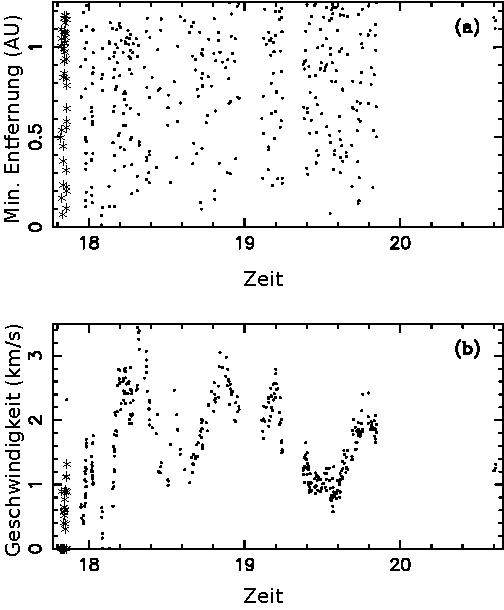
\includegraphics[scale=1]{img/Nesvorny2007-2}
\caption{Die minimalen Abstände und die Geschwindigkeiten von sich nahe kommenden Planeten für Klasse B-Simulation aus Abbildung \ref{fig:Orbitalevolution_vergleich}b. Sterne zeigen Begegnungen zwischen Saturn und Neptun, Punkte stehen für Begegnungen zwischen Uranus und Neptun. Bild nach \cite{Nesvorny2007}.}
\label{fig:Begegnungen}
\end{figure}
Inzwischen sind über hundert irreguläre Monde bei den Gasplaneten bekannt\cite{Nicholson2008}.
Die irregulären Monde bieten wichtige Hinweise zur Entstehungsgeschichte des Sonnensystems und das Verständnis ihrer Entstehung stellte ebenfalls eine Herausforderung dar.
Während sich reguläre Satelliten unseres Wissens durch Akkretion aus der planetaren Gasscheibe gebildet haben, ist die Herkunft von irregulären Monden noch ungeklärt.
Sie müssen auf irgendeine Art von dem Planeten aus einem heliozentischem Orbit eingefangen sein worden. Eine Entstehung aus der planetaren Gasscheibe durch Akkretion wie bei den regulären Monden ist aus mehreren Gründen nicht möglich:
Sie sind von den regulären Trabanten räumlich zu stark getrennt um aus der selben Gasscheibe entstanden zu sein, per Akkretion können keine derartig großen Exzentrizitäten entstehen und vor allem können aus einer Gasscheibe keine retrogard umlaufende Monde entstehen\cite{Nesvorny2007}.

Das System Sonne-Planet-einzufangender Körper reicht jedoch nicht aus, da das System zeitreversibel ist und somit jeder Weg des Körpers von der heliozentischen Bahn zu der Planetenumlaufbahn auch wieder ein möglicher Weg zurück ist\cite{Nesvorny2007}.
Es braucht also einen Mechanismus auf welche Weise ein Trabant dauerhaft eingefangen werden kann. Dazu wurde unter anderem vorgeschlagen, dass der Körper Energie durch Reibung an, den Planeten umgebendes Gas, verliert. % die anderen 2 Modelle erwähnen?
Dieses Modell kann zwar einige der irregulären Moden von Jupiter erklären, nicht jedoch alle, da einige weiter entfernt sind als die Gasscheibe gereicht hat und auch auf die irregulären Monde von Neptun und Uranus lässt sich dieses Modell vermutlich nicht anwenden\cite{Nesvorny2007}. % warum? O-Quelle?
Migrationsmodelle, wie das Nizza-Modell, führen zu einem weiteren großen Problem für derartige \glqq gas-drag\grqq-Modelle. Kommt den so entstandenen irregulären Monden ein großer Planetesimal oder ein Planet zu nahe, werden sie äußerst effizient wieder aus dem System des Planeten gefegt\cite{Nesvorny2007}. Da sich im Nizza-Modell die Planeten Saturn, Uranus und Neptun entsprechend nahe kommen, können die irregulären Monde, die wir heute um diese Planeten sehen, somit nicht aus der Zeit vor der Migration stammen\cite{Tsiganis2005,Nesvorny2007}, was für \glqq gas-drag\grqq-Modelle aber nötig wäre, da zum Zeitpunkt der Migration die Gasscheibe ja sich bereits aufgelöst hat\footnote{Es ist natürlich möglich, dass es früher andere \glqq Generationen\grqq von irregulären Monden gab, welche auf diese Weise entstanden sind, heute aber nicht mehr existieren. }.

Eine weitere wichtige Eigenschaft der irregulären Monde sind ihre vielfältig variierten (von Grau zu starkem Rot) und keinem klaren Gradienten folgenden Farben. Würden die Monde aus der lokalen Umgebung der Planeten stammen, müssten alle Monde eines Planeten eine ähnliche Farbe haben und die Farben der Monde müssten vom Sonnenabstand des Planeten abhängen\cite{Degewij1980Icar,Cruikshank1980Icar,Dumas1998Icar, Sykes2000Icar,Brown2000AJ,Grav2003Icar,Grav2004ApJ,GravHolman2004ApJ,Porco2005Sci,Nesvorny2007}. Dass beides nicht der Fall ist, ist ein Zeichen dafür, dass es sich bei den irregulären Satelliten um ein Mix aus Objekten von ursprünglich unterschiedlichen Orten handelt.

Ein erster Ansatz um irreguläre Satelliten im Rahmen des Nizza-Modells zu erklären wurde 2006 von \cite{Cuk2006} vorgestellt. Dieser geht davon aus, dass irreguläre Monde auf relativ kleinen Bahnen durch \glqq gas-drag\grqq-Modelle entstehen und erst später ihre Bahnen durch die Instabilität des Systems anwächst. Dies konnte die oben angesprochenen Probleme der \glqq gas-drag\grqq-Modelle mit weit entfernten irregulären Monden zumindest bei Saturn – eingeschränkt auch bei Jupiter und Uranus – beheben\cite{Cuk2006}.
Dieses Modell berücksichtigt jedoch nicht, dass es wie oben erwähnt, im Nizza-Modell zu Annäherungen zwischen Planeten kommt, welche derartige irregulären Monde wieder aus ihrer Umlaufbahn werfen würden. Auch die anderen Erkenntnisse legen es nahe, dass die Monde erst während der Instabilitätsphase durch das Einfangen einiger der zahlreichen durch das Sonnensystem fliegenden Planetesimale entstanden.

Als Einfangmechanismus dient hierbei ein dritter massiver Körper,
welcher sich dem Planeten auf weniger als einen Hillradius nähert und Körper,
welche zeitgleich ebenfalls durch den Hillradius fliegen, anregen, so dass einige von ihnen auf stabilen Orbits enden.
Da sich die Gasplaneten nach dem Eintreten der Resonanz näher kommen, während gleichzeitig eine große Anzahl an Planetesimalen das Sonnensystem durchstreift,
ergibt sich folgendes Bild: zwei Planeten kommen sich so nahe, dass sie gegenseitig in den Hillradius des anderen eindringen,
einige der ebenfalls durch den Hillradius der Planeten fliegenden Planetesimale werden dadurch auf weit entfernten Bahnen um einen der Planeten eingefangen und kreisen nun als irreguläre Monde um den Planeten\cite{Nesvorny2007}.
% wohin damit:
In der Ausklingzeit des Nizza-Modells, als die Exzentrizitäten durch dynamische Reibung gedämpft werden und die Scheibe sich langsam leert, ist es möglich, dass die Bahnen der irregulären Monde durch vorbeifliegende besonders massive Planetesmiale (vergleichbar mit den terrestrischen Planeten) noch einmal geändert werden.
Die Existenz derart großer Planetesmiale ist durchaus realistisch, da es keinen Grund gibt, warum sich keine größer Objekte gebildet haben sollen\cite{Nesvorny2007}. Für eine realistische Überprüfung dieses Entstehungsmodell für die irregulären Satelliten muss dieser Effekt also berücksichtigt werden.

Wie oben beschrieben, modellierte die in Nizza ansässige Gruppe die Planetesimalscheibe als eine Scheibe von etwa 1000-5000 gleichschweren Körpern. Dies ist für die Makroskopische Beschreibung des Verhaltens ausreichend, jedoch ist zu erwarten, dass die Scheibe aus wesentlich mehr Teilchen mit unterschiedlichen Massen bestand.
Für die Analyse des hier beschriebenen Einfangprozesses der irregulären Monde, ist die Anzahl der Teilchen von zentraler Rolle, da die Wahrscheinlichkeit eines Einfangs offensichtlich mit der Anzahl der durch das Sonnensystem kreuzenden Planetesimalen steigt.
Die bei den ursprünglichen Simulationen gewählte Anzahl der Planetesimale ist viel zu gering um genügend Einfangprozesse zu beobachten um daraus Rückschlüsse auf die Orbits der eingefangenen irregulären Satelliten und die Effektivität des Einfangprozesses zu machen.
Auf der anderen Seite ist es -- aufgrund der limitierten Rechenzeit -- nicht möglich die Simulation mit der für die Analyse der Einfangprozesse notwendigen Genauigkeit zu berechnen, wenn die Teilchenzahl auch noch erhöht werden soll.
Um dies Problem zu lösen und die Effizienz dieses Einfangprozesses möglichst realistisch zu bestimmen, verwendeten \cite{Nesvorny2007} ein mehrstufiges Verfahren:

Für den ersten Satz von Simulationen, verwendeten sie eine der ursprünglichen Simulationen von \cite{Gomes2005} als Ausgangspunkt.
sie übernahmen die Positions- und Geschwindigkeitswerte aller Objekte zu einem Zeitpunkt kurz vor dem Eintreten der Resonanz und erhöhten dann die Teilchenanzahl der Planetesimalscheibe von einigen hundert auf 6868, %erklären warum nur einige hunder?
ohne die Gesamtmasse oder dynamischen Eigenschaften dieser zu ändern. 50 dieser Systeme, die sich nur durch die genauen Startwerte der einzelnen Planetesimale unterschieden wurden mit SyMBA über Zeitspannen von mindestens 130 Myr simuliert und dabei die Bahnen aufgezeichnet.
Von den sehr unterschiedlich ausfallenden Simulationen wurden im weiteren nur die 14 berücksichtigt, welche ein System lieferten, dass dem unsrigem halbwegs ähnlich war\cite{Nesvorny2007}.
Für diese Simulationen wurden alle Begegnungen von Planeten herausgesucht, bei welchen der Minimalabstand der Planeten kleiner als die Summe der Hillradien der Planeten war.

Im nächsten Schritt wurden dann die Positionen aller Körper von den Zeitpunkten der Begegnung $t_{\mathrm{enc}}$ aus soweit in der Zeit zurückgerechnet, dass sie 5 AU weit von einander entfernt waren  $t_{\mathrm{enc}} - \Delta t$\cite{Nesvorny2007}.
Dafür verwendeten sie nicht SyMBA sondern Bulirsch-Stoer Integrationsalgorithmus, da dieser flexibler ist, wenn es um Simulationen mit großen Teilchenzahlen über nur relativ kurze Zeitspannen geht.

\begin{figure}[tbn]
\centering
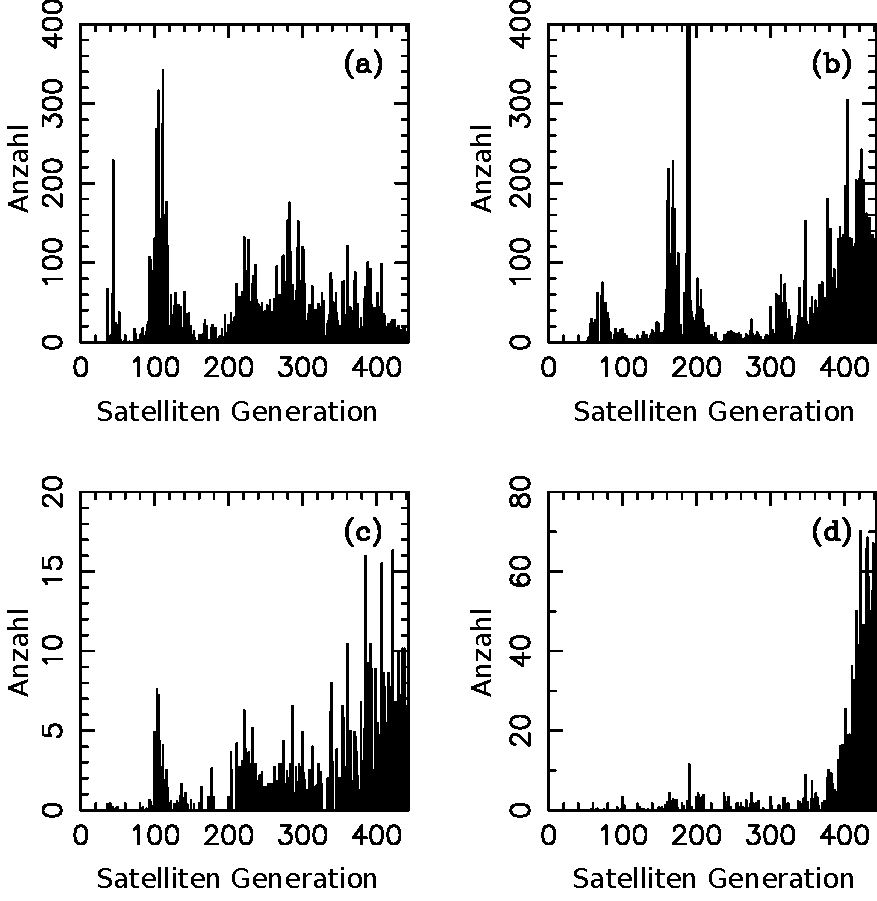
\includegraphics[scale=0.4]{img/Nesvorny2007-8}
\caption{Beitrag der verschiedenen Generationen zum Mondeinfang von Uranus (\textbf{a}), \textbf{b})) und Neptun (\textbf{c}), \textbf{d})). Während in \textbf{a}) und \textbf{b}) nur die Anzahl der eingefangenen Satelliten ohne Berücksichtigung von Wiederentfernungen von Objekten dargestellt ist, sind die in  \textbf{c}) und \textbf{d}) nur die Anzahl der am Ende noch vorhandenen Satelliten aufgetragen. Bild nach \cite{Nesvorny2007}.} %Klammer in Klammer sieht blöd aus
\label{fig:Mondgenerationen}
\end{figure}

\begin{figure}[tbn]
\centering
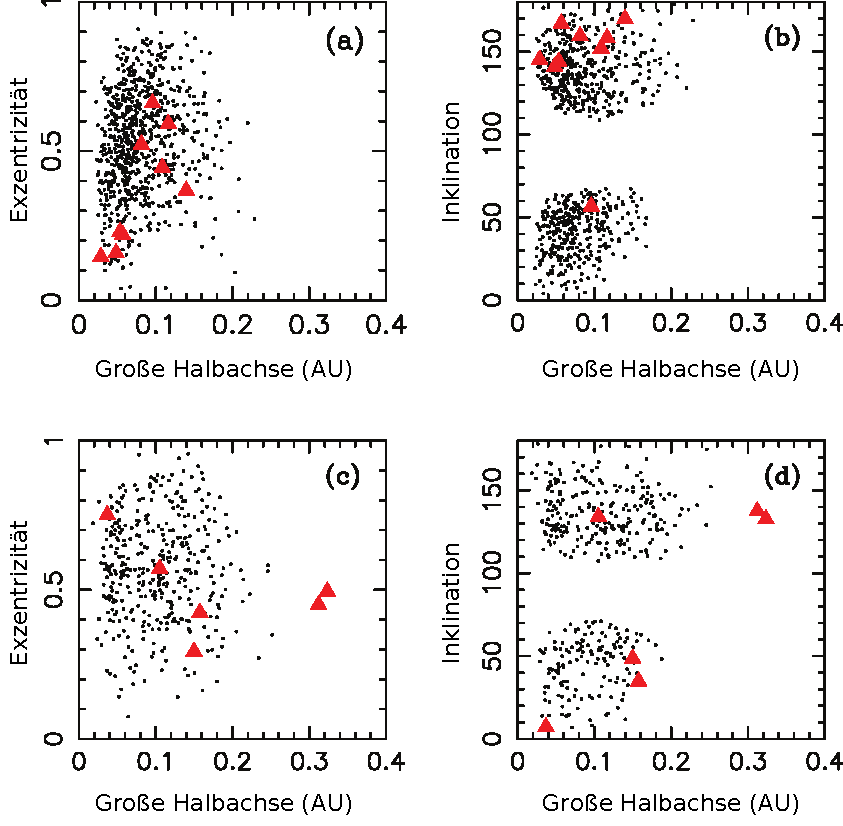
\includegraphics[scale=0.7]{img/Nesvorny2007-4}
\caption{Vergleich der Orbits der Monde einer Simulation der Klasse A mit den Messwerten. Die roten Dreiecke sind die Messwerte der bekannten irregulären Monde, die schwarzen Punkte stellen die in der Simulation gefundenen Monde dar. Abbildungen \textbf{a)} und \textbf{b}) stellen die Satelliten von Uranus, \textbf{c)} und \textbf{d}) die von Neptun dar. Bild nach \cite{Nesvorny2007}.}
\label{fig:KlasseA_Mondorbitale}
%\vspace{\floatsep}
\end{figure}
\begin{figure}[tbn]
\centering
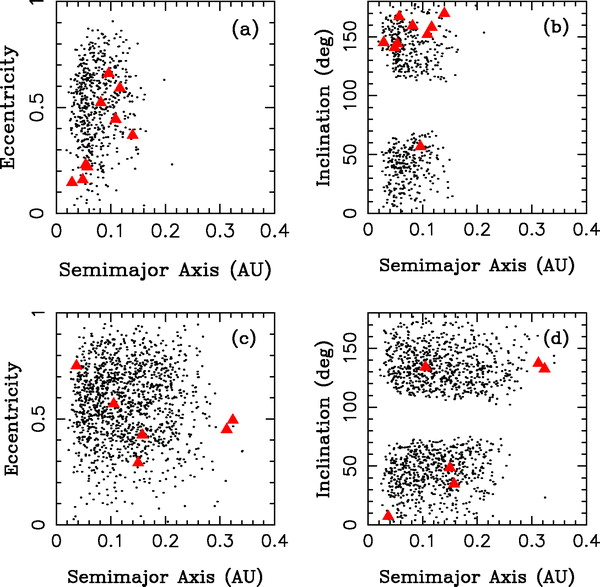
\includegraphics[scale=0.7]{img/Nesvorny2007-5}
\caption{Vergleich der Orbits der Monde einer Simulation der Klasse B mit den Messwerten. Analog zu Abbildung \ref{fig:KlasseA_Mondorbitale}. Bild nach \cite{Nesvorny2007}.} 
\label{fig:KlasseB_Mondorbitale}
\end{figure}

\begin{figure}[tbn] % Bild raus, halb oder ganz verwenden?
\centering
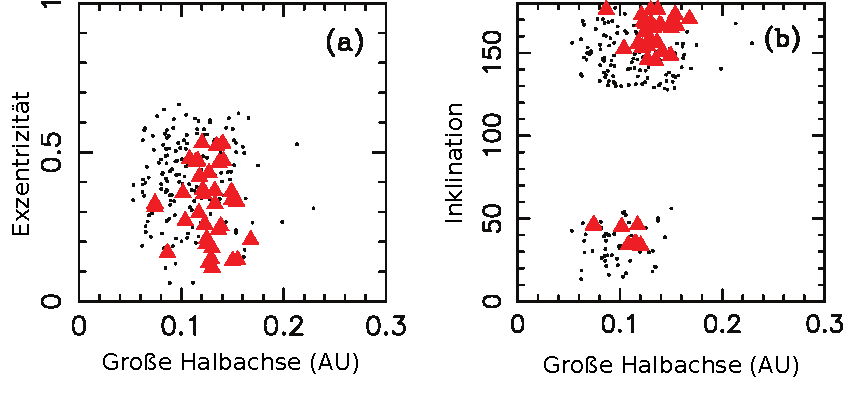
\includegraphics[scale=0.7]{img/Nesvorny2007-6ab}
\caption{Vergleich der Orbits der Saturnmonde der einer Simulation der Klasse B mit den Messwerten. Bild nach \cite{Nesvorny2007}.} 
\label{fig:Saturnmondorbitale}
\end{figure}

\begin{figure}[tbn]
\centering
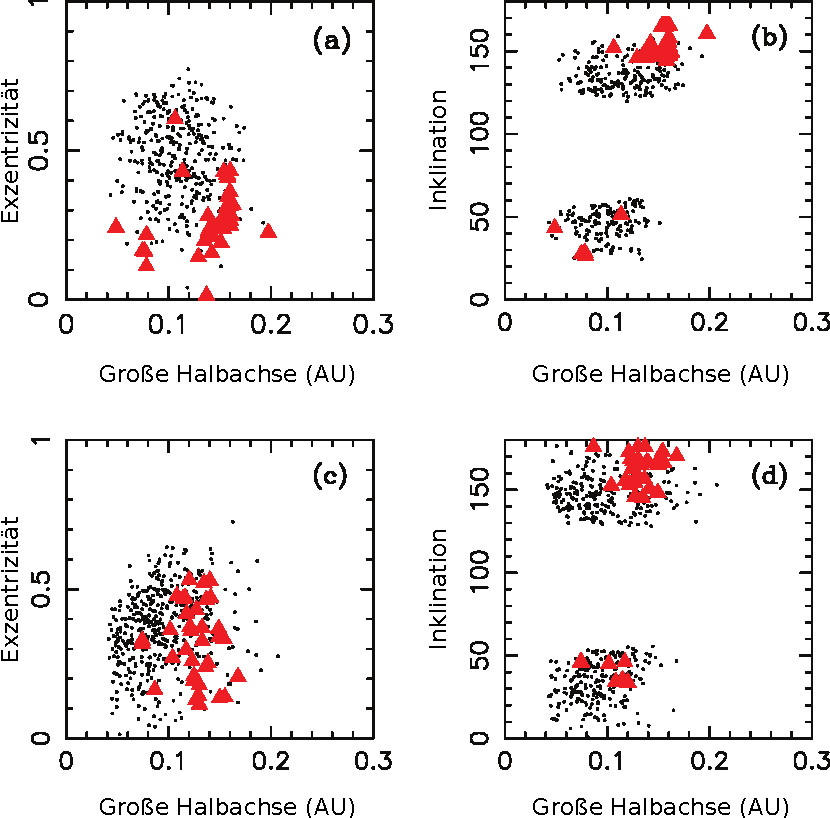
\includegraphics[scale=0.7]{img/Nesvorny2007-7}
\caption{Vergleich der Orbits der Monde der Simulation 9 mit den Messwerten. Abbildungen \textbf{a)} und \textbf{b}) stellen die Satelliten von Jupiter, \textbf{c)} und \textbf{d}) die von Saturn dar. Bild nach \cite{Nesvorny2007}.} 
\label{fig:Sim9_Mondorbitale}
\end{figure}
Im dritten Teil der Simulationen wurden nun die berechneten Werte der Großen Halbachsen, Exzentrizitäten und Inklinationen der Planetesimalen zum Zeitpunkt $t_{\mathrm{enc}}-\Delta t$ verwendet um die Anzahl der Planetesimalen erneut stark zu erhöhen. Man generierte dafür $3 \cdot 10^6$ Teilchen auf zufallsverteilen Orbits, die der Orbitalverteilung der der ursprünglichen Planetesimalen folgten und so gewählt waren, dass sie sich zum Zeitpunkt der Begegnung $t_{\mathrm{enc}}$ in der Nähe der sich begegnenden Planeten sind.
%Die Wahl dieser zufälligen Orbits ist möglich, da es zu diesem Zeitpunkt noch keine resonanten Strukturen in den Planetesimalen gibt.
Nun wurde das erweiterte System über einen Zeitraum von $2 \Delta t$ integriert und die Bahnen anschließend darauf untersucht welche der Planetesimale von einem Planeten eingefangen wurden.
Eine weitere Integration erlaubte es zu testen, ob die eingefangenen Körper stabile Orbits haben oder den Planeten wieder verlassen, bevor es zu einer erneuten Begegnung mit einem Planeten kommt.
Die Simulation der nächsten Planetenbegegnung erfolge identisch, nur dass hier für den Anfangsbedingung zusätzlich auch die Teilchen übernommen wurden die bei der vorherigen Begegnung auf stabilen Orbits um einen Planeten endeten.
Somit wurde berücksichtigt, dass Monde, die derartig bei einer Drei-Körper-Begegnung eingefangen wurden, möglicherweise bei einer erneuten Begegnung von Planeten wieder befreit werden können, sowie, dass es möglich ist, dass ein ursprünglich von einem Planeten eingefangener Mond bei einer erneuten Begegnung zu einem anderen Planeten wechselt, oder seine Bahn verändert\cite{Nesvorny2007}.
Abbildung \ref{fig:Mondgenerationen} zeigt beispielhaft anhand einer Simulation wie viele der endgültig von Uranus und Neptun gefangenen Körper, bei welcher Begegnung eingefangen wurden.
Man erkennt, dass vor allem bei Uranus zahlreiche Generationen zur endgültigen Population beitragen, während bei Neptun nur einige duzend späte Generationen nennenswert beitragen.
Die Berücksichtigung dieser Effekte ist nicht nur für die korrekte Bestimmung der Einfangrate von Bedeutung, auch die Orbits der Monde unterschiedlicher Generationen unterscheiden sich, da die Planetesimalscheibe mit der Zeit immer stärker angeregt wird und die späteren Generationen somit aus einer stärker angeregten Scheibe stammen\cite{Nesvorny2007}.

Abschließend wurden alle nach der letzten Begegnung vorhandenen, gebundenen Teilchen mit einer Simulation über 1 Million Jahre auf ihre lang-zeitliche Stabilität getestet. Dazu verwendeten sie den oben beschriebenen Integrator von \cite{Wisdom1991} in der Version vierter Ordnung.
Dabei wurden zugleich die Durchschnittswerte von Großer Halbachse, Exzentrizität und Inklination der einzelnen Satelliten über die Zeit berechnet.
Für die anschließende Analyse wurden nur die Monde betrachtet die sich in dieser Simulation als stabil erwiesen hatten\cite{Nesvorny2007}.
Bei der Analyse wird auch hier wieder zwischen den beiden Klassen der Migrationsmodelle unterschieden (\refsec{Orbits}).
Von den 14 erfolgreichen Simulationen fielen jeweils 6 auf die beiden Klassen und 2 weitere stellten Mischformen zwischen den beiden dar. Eine Besonderheit stellen die zu Simulationen Nummer 9 und 38 (Klasse B bzw. Mischform) dar, da es bei dieser anders als beim klassischem Nizza-Modell von \cite{Tsiganis2005} auch zu Begegnungen mit Jupiter kam.
Durchschnittlich kam es zu 383 Begegnungen von Planeten, wobei die Anzahl zwischen 55 und 1033 stark schwankte.
Die Anzahl korreliert erwartungsgemäß mit der Gesamtdauer, die die Planeten auf sich kreuzenden Bahnen befinden und ist für die Klasse B höher (473 im Vergleich zu 169 bei Klasse A).
Mit durchschnittlich 345 Begegnungen gab es zwischen Uranus und Neptun die meisten Begegnungen\cite{Nesvorny2007}. %Doppelt
% Bei DE gab es mehr als bei DE <- Problem Klasse A hat per Definition garkeine. Wie rein, doch unterscheiden?
%Die Begegnungen zwischen Saturn und einem Eisgiganten ereigneten sich für gewöhnlich deutlich früher als die zwischen den Eisriesen. % irrelevant?
Die Grafik \ref{fig:Begegnungen} zeigt die Minimalabstände und Geschwindigkeiten der 37 Saturn-Neptun- und 406 Uranus-Neptun-Begegnungen bei einer exemplarischen Simulation.
Das oszillierende Verhalten der Geschwindigkeiten erklären die Autoren nicht.
Auffällig ist dabei auch, dass es nach einer Zeitspanne von fast 800 Tausend Jahren noch einmal 4 Begegnungen gibt\cite{Nesvorny2007}.

Bild \ref{fig:KlasseB_Mondorbitale} zeigt die Orbits der in einer der Simulationen von Klasse B erzeugten Uranus- und Neptun-Monde im Vergleich mit den heute real existierenden.
Die Werte für Uranus (\ref{fig:KlasseB_Mondorbitale}a, \ref{fig:KlasseB_Mondorbitale}b) stimmen bemerkenswert gut überein, wobei es auch hier zwei Abweichungen gibt.
Zum einen ist die Verteilung der Inklinationen der retrograd laufenden Satelliten in Realität wie in der Grafik zu sehen dichter und etwas größer als in der Simulation, 
zum anderen – und das ist der größere Unterschied zwischen Modell und Realität – sind im Modell normal und rückwärtslaufende Trabanten etwa gleich häufig, während in Realität acht der neun Monde eine retrograde Bahn haben\cite{Nesvorny2007}.
Die zu niedrige Inklination könnte durch die Verwendung einer dynamisch kältereren Planetesimalscheibe oder durch eine Veränderung des Modells zugunsten der stärkeren Bedeutung früherer Generationen eingefangener Satelliten korrigiert werden\cite{Nesvorny2007}.
Die Asymmetrie zwischen normal und rückwärtslaufenden irregulären Monden ließe sich durch Kollisionen zwischen diesen beiden Gruppen erklären, welche in den Simulationen von \cite{Nesvorny2007} nicht berücksichtigt wurden. So könnte Sycorax – der größte retrogarde, irreguläre Mond von Uranus (Durchmesser von etwa 190 km) – mehrere kleinere progarde Monde zerstört haben\cite{Nesvorny2007}.
Für Neptun (\ref{fig:KlasseB_Mondorbitale}c, \ref{fig:KlasseB_Mondorbitale}d) stimmen die Resultate ebenfalls sehr gut überein, jedoch nur für 4 der 6 Monde, die Monde Neso und Psamathe haben deutlich größere Entfernungen von Neptun als die anderen\cite{Nesvorny2007}.
Simulationen der Klasse A können diese gar nicht erklären (Abbildung \ref{fig:KlasseA_Mondorbitale}), für Simulationen der Klasse B waren derartig große Entfernungen zwar ungewöhnlich, kamen jedoch vor.
Der Unterschied zwischen den beiden Klassen bezüglich der maximal auftretenden großen Halbachsen liegt daran, dass die sogenannte \glqq evection ressonance\grqq\ -- eine Resonanz zwischen der Apsidendrehung des Satelliten und der Bahnbewegung des Planeten -- zu starken Instabilitäten für Bahnen mit $a \gtrsim \frac{1}{2} R_H$ führt\cite{Nesvorny2003,Nesvorny2007}.
Der Hillradius eines Planeten wächst jedoch mit wachsender Entfernung von der Sonne und da bei der Klasse A Neptun zum Zeitpunkt der letzten Begegnung noch eine deutlich kleinere Bahn hat sind die großen Halbachsen seiner Monde auf $a < \unit[0,26]{AU}$ beschränkt\cite{Nesvorny2007}.
Auch dies ist ein Vorteil von Klasse B, wobei es auch Möglichkeiten gäbe Neso und Psamathe durch Streuung – zum Beispiel durch den Einfang von Triton (vermutlich durch einen anderen Mechanismus) – auf ihre heutigen Bahnen zu bringen. % Sonderrolle von Triton erläutern?
Fünf der 14 Simulationen erzeugten keine oder nur einen Trabanten um Saturn, bei den restlichen stimmten die Orbitalverteilung der Satelliten mit der der realen Planeten sehr gut überein, siehe \ref{fig:Saturnmondorbitale}\cite{Nesvorny2007}.
In der schon oben erwähnten Simulation Nr. 9 (Abbildung \ref{fig:Sim9_Mondorbitale}), in welcher es auch Planetenbegegnungen mit Jupiter gab, bekam auch dieser zahlreiche Trabanten (341 Stück), welche ebenfalls gut zu den beobachteten irregulären Monden passen. Dabei treten ähnliche Probleme wie bei Uranus auf, insbesondere was die zu kleinen Inklinationen der retrograden Monde angeht.
Zu Jupiter sollte noch angemerkt werden, dass bekannt ist, dass die meisten Monde auf rückläufigen Bahnen Fragmente von Kollisionen einiger größeren Monde sind, was den Vergleich der Orbits erschwert\cite{Nesvorny2004,Nesvorny2007}.

\begin{figure}[tbn]
\centering
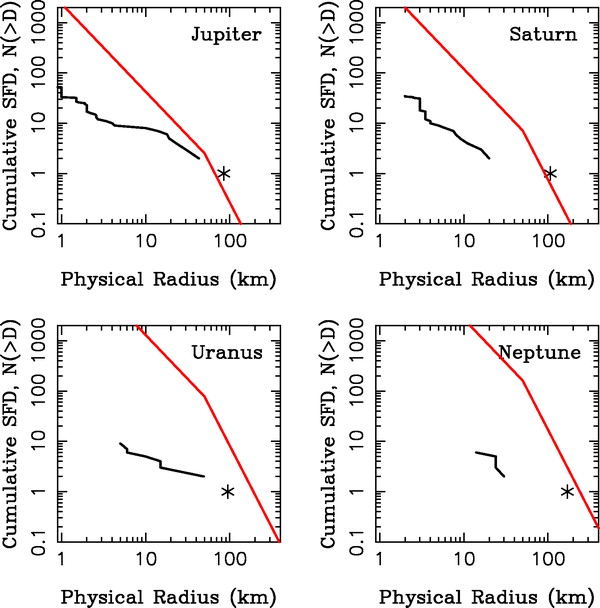
\includegraphics[scale=.5]{img/Nesvorny2007-9}
\caption{Size-frequency distribution (SFD) wie im Modell berechnet (rote Linie) und gemessen (schwarzer Strich, beziehungsweise Sternchen für den jeweils größten Mond). Bild nach \cite{Nesvorny2007}.}
\label{fig:SFD}
\end{figure}
Nachdem die Teilchenanzahl in den Simulationen möglichst hoch gewählt wurde um möglichst genaue Aussagen über die Orbits der Monde treffen zu können, 
soll nun mit realistischeren Werten überprüft werden, inwieweit die Anzahl der durch das Modell erzeugten irregulären Monde mit der beobachteten übereinstimmt.
Dafür bestimmten \cite{Nesvorny2007} die Einfangwahrscheinlichkeit für einen Planetesimal durch einen Planeten.
Die Einfangquote eines Satelliten in einer Simulationen berechnet sich durch:
\begin{equation}
P_{\mathrm{capture}} = \sum\limits^{N_{\mathrm{enc}}}_{j=1} \frac{N_{\mathrm{sat}; j}}{N_{\mathrm{test}}}\cdot \frac{N_{\mathrm{activ}; j}}{N_{\mathrm{total}}}
\end{equation} % eindeutschen!? besser setzen!
dabei ist $N_{\mathrm{enc}}$ die Anzahl der Begegnungen mit anderen Planeten, $N_{\mathrm{sat};j}$ die Zahl der bei der j-ten Begegnung erzeugten Satelliten, $N_{\mathrm{test}} = 3 \cdot 10^6$ die Zahl der jeweils für die Begegnung injizierten Testteilchen, 
$N_{\mathrm{active}; j}$ ist die Anzahl an Teilchen bei der Ausgangssimulation in der Nähe der sich nahe kommenden Planeten waren und als Klonvorlage für die injizierten Testteilchen dienten und $N_{\mathrm{total}} = 6868$ ist die Anzahl der in der ersten Simulation anfangs verwendeten Planetesimale\cite{Nesvorny2007}.
Die Durchschnittswerte der so berechneten Einfangswahrscheinlichkeit für Uranus und Neptun betragen $2,6 \cdot 10^{-7}$ beziehungsweise $5,4 \cdot 10^{-7}$.
Für Saturn und vor allem für Jupiter macht das Betrachten des Durchschnittswertes aufgrund der großen Schwankungen wenig Sinn, hier verwendenden die Autoren die bei Simulation 9 auftretenden Maximalwerte von $8,5 \cdot 10^{-9}$ beziehungsweise $2,4 \cdot 10^{-8}$\cite{Nesvorny2007}.
Die Werte für $P_{\mathrm{capture;Saturn}}$ sind für Simulationen der Klasse B meist höher\cite{Nesvorny2007}.
Nachdem wir aus den Simulationen von \cite{Tsiganis2005} wissen, dass die Gesamtmasse der Planetesimalscheibe $\approx\unit[35]{\ME}$ betragen muss (\refsec{Orbits}),
brauchen wir zur Bestimmung der Anzahl und Größe der irregulären Monde noch die size-frequency distribution (SFD) der Planetesimalscheibe.
Da das Nizza-Modell – wie wir in Kapitel \ref{Kuiper} besprechen werden – davon ausgeht, dass die Überreste der Planetesimalscheibe den heutigen Kuipergürtel darstellt und es nach dem LHB nur relativ wenige Veränderungen der SFD durch Kollisionen im Kuipergürtel gab, gehen die Autoren davon aus, dass die SFD des Kuipergürtels der der Planetesimalscheibe entspricht\cite{Nesvorny2007}.
Die SFD des Kuipergürtels entspricht in erster Näherung zwei Potenzfunktionen, für kleine Durchmesser folgt der SFD einer Potenzfunktion mit Exponenten $q_2 \approx 2-3$ während bei großen Durchmessern die SFD mit $q_1 \approx 4-4,5$ abfällt, wobei der Übergang bei etwa $D \approx 100$ Kilometern oder etwas darunter liegt\cite{Gladman2001,Trujillo2001a,Bernstein2004,Petit2006,Nesvorny2007}.
Wählt man $q_2 = 2,75$, $q_1 = 4,25$ und $D = 100$ bei einer Planetesimalscheibenmasse von $\unit[35]{\ME}$ erhält man mit den  Einfangswahrscheinlichkeiten die in Abbildung \ref{fig:SFD} rot gezeigten kumulierten SFDs für die eingefangenen Monde der vier Planeten.
Beim Vergleich mit den schwarz eingezeichneten SFD der gemessenen irregulären Monde,
stellt man einige Abweichungen fest:
Uranus und Neptun haben in Realität deutlich weniger irreguläre Monde als hier vorhergesagt,
Jupiter und Saturn haben deutlich zu viele kleine Monde und die SFD des Modells (gleich der des Kuipergürtels) ist allgemein für Mondradien von $D\gtrsim 10 \, \mathrm{km}$ deutlich steiler als in Realität (Exponent von $\approx2$)\cite{Nesvorny2007}.
Dies sind einerseits große Diskrepanzen zwischen Modell und Realität, jedoch ist die Tatsache, dass mehr Monde vorhergesagt werden nur ein kleines Problem, es wäre ein deutlich größeres Problem, wenn das Modell zu wenige Monde erzeugen würde. Der Autor gibt einige Effekte an, welche diese Diskrepanzen erklären könnten:
\begin{itemize}
\item Die SFD der Planetesimalscheibe zum Zeitpunkt des Einfangs könnte doch anderes sein und sich erst später zu der des Kuipergürtels entwickeln.
So könnte sie früher flacher sein und sich erst später durch Kollisionen verändert haben. Dies würde sich jedoch nur schlecht mit anderen Aussagen des Nizza-Modells wie der Erklärung des LHBs oder der Existenz von Plutoiden vertragen, % erklären warum? Nesvorny2007 S.74 rechts oben
weshalb \cite{Nesvorny2007} dies als ungeeignete Erklärung ablehnen.
Eine Reduzierung der Anzahl eingefangener Objekte wäre jedoch möglich, wenn ein größerer Massenanteil sich auf sehr kleine oder sehr große Objekte verteilen würde\cite{Nesvorny2007}. % erklären warum von Bedeutung!, Diskussion
\item Durch Kollisionen zwischen Monden kann sich die SFD und die Anzahl der Monde verändern. Während des LHB durchdringen zahlreiche Planetesimale die Hillsphäre der Planeten und können dabei mit Monden kollidieren oder diese von ihrer Bahn bringen\cite{Nesvorny2007}. Durch diese Effekte könnten die meisten Monde zerstört werden und sich die SFD entsprechend ändern. Simulationen die diese Effekte berücksichtigen wären möglich, sind mir jedoch nicht bekannt. % nochmal suchen!
\item Beim Einfang von Triton könnten Neptun-Monde verloren gegangen sein, was jedoch die Diskrepanz bei Uranus unberührt lassen würde\cite{Nesvorny2007}.
\item Es könnte noch mehr irreguläre Monde geben, die nur noch nicht gefunden wurden. So wurden in den 2000er Jahren durch das aufkommen von großformatigen CCD Detektoren jährlich einige Monde entdeckt und Hochrechnungen gehen davon aus, dass jeder der Riesenplaneten etwa 100 irreguläre Monde mit Durchmessern größer als 1 Kilometer  hat\cite{Nicholson2008}.
Ein \glqq Wachstum\grqq\ um zwei ganze Größenordnungen -- wie es zur alleinigen Erklärung der Diskrepanz Notwendig wäre -- ist jedoch sicherlich nicht anzunehmen.
\end{itemize}

Auch wenn diese Probleme beseitigt werden können, so bleibt die Frage der Interpretation der irregulären Monde von Saturn und vor allem Jupiter. In beiden Fällen sind selbst die maximalen Einfangseffizienzen kleiner als die durchschnittlichen Effizienzen bei Uranus und Neptun,
während in Wirklichkeit alle Planeten ähnlich große Populationen von irregulären Monden haben\footnote{Bei Jupiter und Saturn sind sogar wesentlich mehr irreguläre Monde bekannt, dies ist aber Effekt durch die verzerrte Bobachtbarkeit.}\cite{Nesvorny2007}. % verzerrte Bobachtbarkeit
Jupiter begegnet im ursprünglichen Nizza-Modell den anderen Planeten gar nicht.
Simulation Nummer 9 hat jedoch gezeigt, dass dem nicht notwendigerweise so ist und es durchaus möglich wäre, dass auch Jupiter seine irregulären Monde derart eingefangen hat.
Allerdings war diese Simulation eine seltene Ausnahme – in nur 2 der 14 erfolgreichen Simulationen kam es zu Planetenbegegnungen mit Jupiter und nur in dieser einen wurden auch Planetesimale eingefangen.
Eine Modifikation der Anfangsbedingung des Nizza-Modells könnte die Zahl der Planetenbegegnungen mit Beteiligung von Jupiter oder Saturn erhöhen -- wie wir in Kapitel \ref{jumpingjupiter} sehen werden, gibt es inzwischen eine Modifizierte Version des Nizza-Modells welche dies erfüllt und auch aus anderen Gründen Vorteile bringt.
Alternativ könnte man die These aufstellen, dass die irregulären Monde von Jupiter und Saturn – zumindest teilweise – auf andere Weise entstanden. Da diese Planeten je nach Simulationstyp nicht, beziehungsweise seltener, anderen Planeten nahe kommen, fällt für sie das Argument weg, sie könnten nicht vor dem LHB entstanden sein, da sie sonst bei Planetenbegegnungen verloren gegangen seien.
Ein Argument dafür ist, dass es im Gegensatz zu den irregulären Monden von Uranus und Neptun, zwischen einigen der Monde von Jupiter und Saturn Resonanzen gibt, die darauf hindeuten, dass diese Monde schon viel älter als das LHB sind\cite{Beauge2007,Nesvorny2007}.
Allerdings ließen sich damit die oben angesprochenen Ähnlichkeiten der Populationen aller vier Planeten nicht erklären.

\FloatBarrier
\section{Kuipergürtel}\label{Kuiper}
\begin{figure}
\centering 
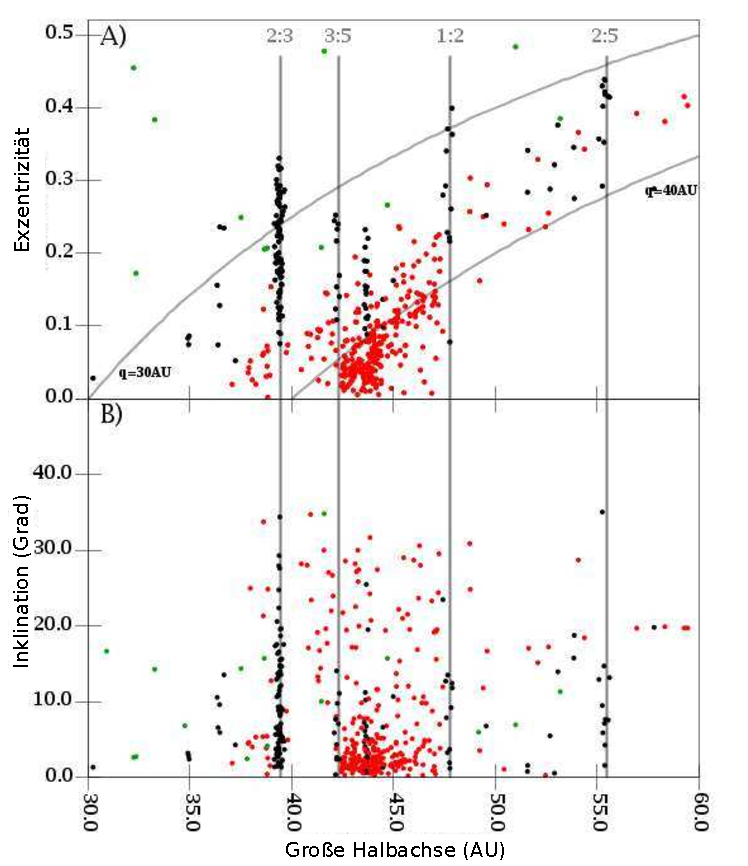
\includegraphics[scale=0.7]{img/LEVISON2008-1-mod}
\caption{Darstellung der Transneptunischen Objekte. Man erkennt neben dem Klassischen Kuipergürtel die Resonanten KBOs -- insbesondere die Plutinos -- und die Gestreuten KBOs. Nicht mehr im Bild sind die Detached Objects und die Oortsche Wolke. Bild nach \cite{Levison2008}.}
\label{fig:KBOs}
\end{figure}
\begin{figure}
\centering 
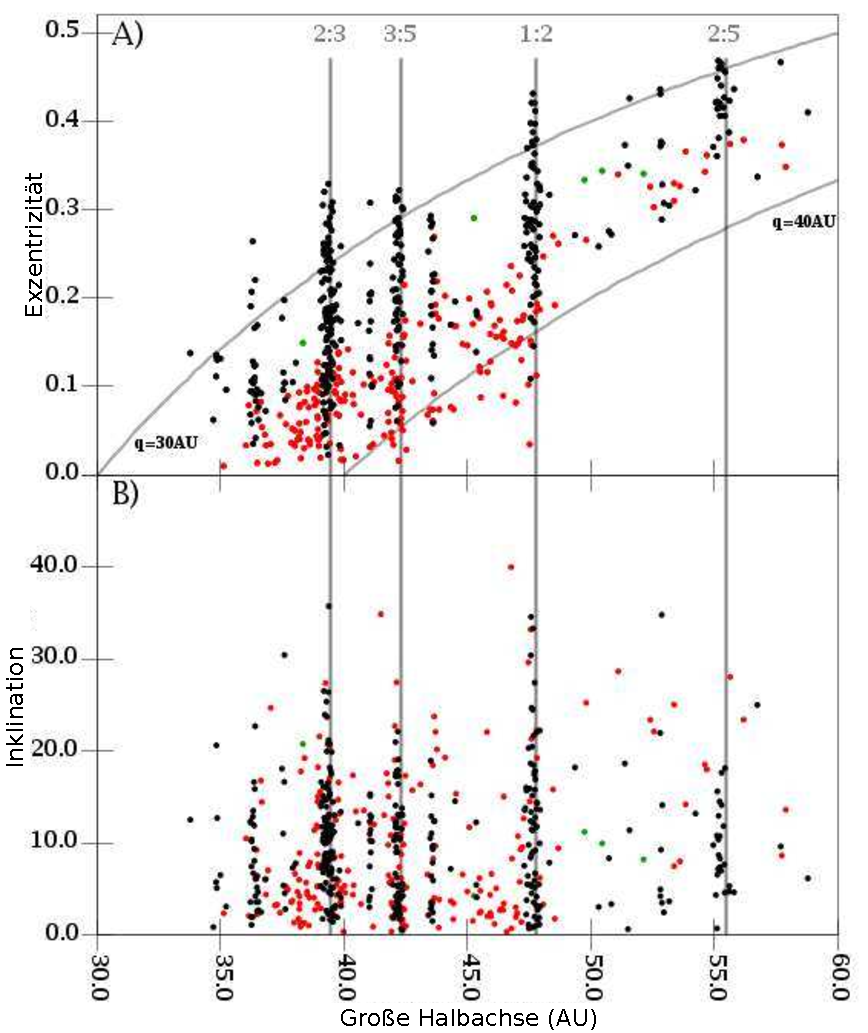
\includegraphics[scale=0.7]{img/LEVISON2008-6-mod}
\caption{Darstellung der Transneptunischen Objekte, in einer der Simulationen von \cite{Levison2008}. Die Übereinstimmung mit Abbildung \ref{fig:KBOs} ist deutlich sichtbar. Bild nach \cite{Levison2008}.}
\label{fig:KBOs_sim}
\end{figure}
Als Transneptunische Objekte (TNO) bezeichnet man alle Himmelskörper, die außerhalb der Neptunbahn um die Sonne kreisen. Die meisten dieser Objekte sind Teil des bekannten Kuipergürtels, zuweilen werden auch alle Transneptunischen Objekte zusammen als Kuiperbelt Objects (KBOs) bezeichnet.
Die wichtigsten Untergruppen der TNOs sind:
\begin{itemize}
\item Resonante KBOs: Objekte die sich in einer MMR zu Neptun befinden. Die bekanntesten Gruppen dieser sind die auf der 2:3-MMR liegenden Plutinos\footnote{Nicht zu verwechseln mit Plutoiden, womit alle transneptunischen Zwergplaneten bezeichnet werden.} -- zu denen das Pluto-Charon-System gehört -- sowie die Twotinos mit einer 1:2-Resonanz zu Neptun. Daneben gibt es jedoch noch zahlreiche weitere (3:5, 4:7, 2:5), welche in einem Plot der Exzentrizität über die Große Halbachse wie in Bild \ref{fig:KBOs} deutlich auffallen\cite{Levison2008}.
Die Schätzungen darüber wie viele der Objekte in einer Ressonanz zu Neptun stehen gehen deutlich auseinander, 
so schätzt sie \cite{Trujillo2001,Levison2008} auf etwa 10\%, während \cite{Kavelaars2008,Levison2008} alleine den Anteil der Plutions auf etwa 20\% schätzt.
\item Klassische KBOs (CKBO) oder Cubewanos: Als den Klassischen Kuipergürtel, bezeichnet man die nicht resonanten Objekte, die sich auf stabilen, nahezu kreisförmigen Bahnen mit Großen Halbachsen kleiner als 48 AU befinden.
\item Gestreute KBOs (SKBO, Scattered Disk Objects, SDO) haben noch deutlich größere Große Halbachsen und sehr hohe Exzentrizitäten und Inklinationen. Ihren Namen haben sie daher, dass sie durch Streuung auf ihre Bahnen gekommen sein müssen.
\item Detached Objects oder Extended Scattered Disc Objects (ESDO): Dabei handelt es sich um noch weiter entfernte Objekte -- ihr Perihelion ist so weit vom gravitativen Einfluss von Neptun entfernt, dass sie durch diesen und die anderen Planeten nicht beeinflusst werden. Als bekanntes Mitglied der Detached Disk gilt meist Sedna, die Gruppe um Levison hingegen geht jedoch davon aus, dass Sedna Prototyp einer weiteren neuen Klasse von Objekten ist\cite{Morbidelli2004,Kenyon2004,Brasser2006,Levison2008}.
\item Objekte der Oortschen Wolke. Die von Jan Oort und Ersnt Öpik 1950 postulierte Wolke in einer Entfernung von mehreren Tausend AU ist der Ursprung der Kometen. Sie wird in eine innere Oortsche  Wolke (2.000–20.000 AU) und einer äußeren Oortsche Wolke (20.000–50.000 AU oder noch weiter) geteilt. Sedna wird manchmal als Teil der inneren Oortschen Wolke betrachtet – \cite{Brasser2008} verwendet den Begriff innerste Oortsche Wolke als Bezeichnung für die hypothetische Population zu welcher Sedna gehört. Da dies mit der im letzten Punkt genannten Einschätzung Levisons deckt, werde ich dies im folgenden übernehmen.
\end{itemize}

\noindent
Bei den Transneptunischen Objekten handelt es sich -- unabhängig vom Nizza-Modell -- um ein Relikt aus der Zeit der Planetenentstehung. Die Entwicklung des Sonnensystem schlug sich in den Eigenschaften der TNO nieder, so das sie eine wichtige Informationsquelle für die Geschichte des Sonnensystems und ein Testobjekt für neue Modelle darstellen.
So weisen die Transneptunischen Objekte einige interessante Eigenarten auf, die ein Modell der planetaren Evolution erklären können sollte:
\begin{enumerate}
\item Die Existenz und der große Anteil der Resonanten KBOs: Einige der Resonanten KBOs weisen eine Libration auf. Die Librationsamplitude ist neben Exzentrizität und Inklination dann eine weitere wichtige Bahneigenschaft, deren Verteilung von einem Modell erklärt werden muss. Dies gilt insbesondere für die sogenannten 2:5-Libratoren\cite{Levison2008}. % Libration definieren
\item Die Klassischen Kuipergürtel-Objekte haben eine mittlere Exzentrizität von etwa 0.07, was zwar klein, jedoch trotzdem um eine Größenordnung größer als zur Zeit der Entstehung ist. Da die Obergrenze der Exzentrizität der CKBOs durch Bahnstabilitätsgründe vorgegeben ist, ist sogar anzunehmen, dass es früher Objekte mit noch deutlich höherer Exzentrizität gab.
\item Transneptunische Objekte mit fast kreisförmiger Bahn gibt es nur für Große Halbachsen bis zu etwa 44 AU, danach steigt die Exzentrizität mit der Entfernung an (siehe Bild \ref{fig:KBOs})\cite{Levison2008}. Dieses Resultat scheint kein Effekt mangelnder Beobachtungsdaten für höhere Entfernungen sondern eine reale Eigenschaft der TNO zu sein\cite{Levison2008}.
\item Der klassische Kuipergürtel endet genau am Ort der 1:2-MMR mit Neptun\cite{Levison2008}. Auch dies kann nicht durch Verzerrungen durch mangelnde Beobachtungsfähigkeiten für weit entfernte Objekte erklärt werden.
\item In a-i-Diagramm in Bild \ref{fig:KBOs} erkennt man, dass es zahlreiche Objekte mit sehr kleiner Inklination ($i\lesssim 4^\circ$), jedoch auch etliche mit größeren Inklinationen (bis zu $\sim 30^\circ$) gibt. Berücksichtigt man hier die Verzerrung durch die Beobachtbarkeit -- welche etwa zu $1/\sin(i)$ proportional ist -- so stellt man fest, dass sich die Objekte in zwei Cluster einteilen lassen und die Inklinationsverteilung durch zwei überlagerte Gaussverteilungsfunktionen gefittet werden kann\cite{Brown2001,Levison2008}.
Man nennt die Population mit den geringen Inklinationen die \glqq kalte Population\grqq\ und die mit den großen Inklinationen die \glqq heiße Population\grqq. Obwohl wir von der kalten Population wesentlich mehr Objekte kennen, ist die heiße Population in Wirklichkeit die größere\cite{Levison2008}.
\item Es fällt auf, dass es Zusammenhänge zwischen den Orbitaleigenschaften und physikalischen Eigenschaften der Objekte gibt. So sind helle Objekte in der kalten Population deutlich unterrepräsentiert\cite{Levison2001a}. Gleichzeitig konnte gezeigt werden, dass die Objekte der kalten Population größere Albedos haben, somit sind die Objekte der heißen Population deutlich größer als die der kalten\cite{Grundy2005}.
Darüber hinaus zeigten mehre verschiedene Arbeiten \cite{Tegler2000,Doressoundiram2001,Trujillo2002,Doressoundiram2005,Elliot2005,Levison2008}, dass die heiße Population ein breites Farbspektrum von rot bis grau haben, während die kalte Population fast nur aus roten Objekten besteht.
Auch Objekte mit sehr großer Apoheldistanz sind einheitlich rot, unabhängig von ihrer großen Halbachse.
Allgemein scheint es eine Beziehung zwischen der Farbe und der Periheldistanz zu geben: graue Objekte werden für kleinere q häufiger.
\item Die Objekte der detached disk können nicht durch die Planeten auf ihren heutigen Orbits auf ihren heutigen Bahnen auf ihre Orbits gelangt sein, da sie außerhalb des Einflussbereichs dieser sind\cite{Levison2008}.
\item Ein besonders großes Problem ist das Massendefizit des Kuipergrütels. Die Masse des Kuipergürtels wird auf $\unit[0.01]{\ME}$ bis $\unit[0.1]{\ME}$ geschätzt\cite{Gladman2001, Bernstein2004, Levison2008}.
Damit sich aus dem Material jedoch innerhalb einer vernünftigen Zeitspanne von $10^7-10^8$ Millionen Jahren die Objekte mit der heutigen Größe zusammenklumpen konnten, musste es $10$ bis $\unit[30]{\ME}$ festes Material in der dynamisch Kalten Scheibe geben.\cite{Stern1996AJ, Stern1997AJ, Stern1997ApJ, Kenyon1998AJ, Kenyon1999AJ, Kenyon1999ApJ, Kenyon2004}
\end{enumerate}

\noindent
Im Rahmen des Nizza-Modells werden die TNO als die Überbleibsel der Planetesimalenscheibe betrachtet.
Um dies zu überprüfen, führten \cite{Levison2008} weitere, dafür optimierte Simulationen durch. Als Integratoren  dienten hier die Kombination von zwei Varianten des Swift-Codes, einmal mit dem oben diskutierten Mapping von \cite{Wisdom1991} und einmal mit dem nicht symplektischen Algorithmus RMVS von \cite{Levison1994}. Auch hier wurde, wie bei den Simulationen zur Untersuchung des LHBs, die Migration der Planeten durch Hinzufügung geeigneter Kräfte auf das System erzwungen und die Planetesimale wurden nur als Testteilchen behandelt\cite{Levison2008}.
Die Simulationen beinhalteten 60.000 Planetesimale und erstreckten sich jeweils über einen Zeitraum von einer Milliarde Jahren\cite{Levison2008}. Die Gruppe um Levison führte fünf derartige Simulationen durch, wofür sie insgesamt 2 CPU-Jahre Rechenzeit brauchten – eine vollständige Untersuchung des Parameterraums ist deshalb nicht möglich gewesen\cite{Levison2008}.
Mit diesen Simulationen ergibt sich folgendes Bild:
Wenn Neptun migriert, steifen die Positionen seiner MMRs durch die Planetesimalenscheibe. Da die MMRs von Neptun ''klebrig`` sind\cite{Levison2008}, werden Objekte über welche die MMRs streifen eingefangen und bilden seitdem die Resonanten Kuipergürtel Objekte. Auch Pluto kam so auf seine heutige Bahn.
Zur Zeit als Neptuns Exzentrizität größer als $\sim 0,15$ war, überlappten sich laut numerischen Berechnungen die MMRs, so dass der Bereich zwischen Neptuns Orbit und seiner 1:2 MMR ein Gebiet ergibt, in welchem sich Teilchen frei Bewegen können, sie können jedoch nicht über die 1:2 MMR hinaus wandern\cite{Levison2008}. Dies erklärt warum der Kuipergürtel durch diese Resonanz begrenzt ist.
Die kalte und die heiße Population des Kuipergürtels wurden dabei durch zwei unterschiedliche Mechanismen auf ihre heutigen Orbits gebracht und stammen deshalb aus unterschiedlichen Bereichen der Planetesimalenscheibe. Die kalte Population stammt aus Objekten mit einer größeren Sonnendistanz, was zumindest erklären würde, warum es weniger graue Objekte gibt. Um zu erklären, dass es praktisch gar keine grauen Objekte in der kalten Population gibt, vermuten die Autoren, dass nicht nur der Entstehungsort sondern auch seine spätere Entwicklung die Farbe prägt\cite{Levison2008}.
Einige der Objekte werden durch Interaktionen mit verschiedenen Resonanzen Neptuns weiter hinaus gestreut und bilden so die Scatered Disk\cite{Levison2008}.
Der Massendefizit erklärt sich qualitativ trivial dadurch, dass nur ein kleiner Anteil der Planetesimale auf stabilen Bahnen im Kuipergürtel enden. Quantitativ ergaben sich in den Simulationen von \cite{Levison2008} eine Masse des klassischen Kuipergürtels von zwischen $\sim\unit[0.05]{\ME}$ und $\sim\unit[0.14]{\ME}$, was gut mit den Messwerten übereinstimmt.
Die Ergebnisse einer ihrer Simulationen sind in Abbildung \ref{fig:KBOs_sim} dargestellt, die Übereinstimmung mit Abbildung \ref{fig:KBOs} ist deutlich.

Insgesamt konnten \cite{Levison2008}mit ihren Simulationen zeigen, dass das Nizza-Modell alle obengenannten Punkte bis auf einen erklärt: Die Durchschnittsexzentrizität des klassischen Kuipergürtels in den Simulationen betrug 0.10-0.13, während sie in Realität 0.07 beträgt.
Die Autoren weisen darauf hin, dass dies aufgrund der geringen Zahl der Simulationen eine statistische Schwankung sein könnte, oder auf den nicht ganz abgedeckten Parameterraum zurückzuführen sein könnte. Auch wäre es möglich, dass in der Simulation nicht berücksichtigte physikalische Effekte wie die durch Kollisionen verursachte Dämpfung der Exzentrizität diese Diskrepanz verursachen\cite{Levison2008}.
Nur durch eine deutliche Vergrößerung der Rechenleistung oder aber effizientere Simulationen wird man dies überprüfen können.

Auf ein weiteres Problem wies \cite{Parker2010} hin:
Etwa 30 Prozent der Objekte der Kalten Population des Klassischen Kuipergürtels sind Doppelsysteme wie das Pluto-Charon-System.
Viele von ihnen sind nur sehr lose aneinander gebunden und würden deshalb die Interaktionen mit Neptuns Resonanzen nicht überleben.

Trotz dieser Probleme, ist der Grad an Übereinstimmung der beobachten Kuiper\-gürtel\-eigen\-schaften mit den Ergebnissen des Nizza-Modells beeindruckend und bisher von keinen anderem Modell erreicht.
Ein weiterer positiver Aspekt ist, dass das Nizza-Modell auch erklärt warum die Jupiter-Trojaner den Objekten des Kuipergürtels im optischem sehr ähnlich sehen, schließlich haben nach diesem Modell beide denselben Ursprung\cite{Morbidelli2005}.

Während die durch Sedna repräsentierte innerste Oortsche Wolke bereits in den Anfangszeiten des Sonnensystems entstanden sein kann, ist die Erklärung der restlichen Oortschen Wolke mit bisherigen Modellen schwerer – die bisherigen Modelle versuchten diese durch die Wechselwirkung von am Sonnensystem vorbei fliegenden Sternen zu erklären, ergaben jedoch zu geringe Massen – daher untersuchte \cite{Brasser2008} ob die zerstreute Planetesimalscheibe im Nizza-Modell nicht auch Ursprung der Oortschen Wolke sein kann.
Er schlägt daher ein zweistufiges Verfahren vor, in welchem die innerste Oortsche Wolke mit einem der bereits vorgeschlagenen Modelle (\cite{Brasser2006,Brasser2007} oder \cite{Kaib2008}) entstand, während die innere und äußere Oortsche Wolke ein Gyr später – zeitgleich zum LHB – durch einen von \cite{Dones2004} bereits 2004 vorgeschlagenen Mechanismus aus den selben Planetesimalen, die auch das LHB auslösten, entstanden\cite{Brasser2008}.
Er bestimmte die Masse der dadurch gebildeten äußeren Oortschen Wolke auf etwa $\unit[0.5]{\ME}$, was etwas weniger als die $\unit[0.6-1.4]{\ME}$ sind, auf die die Messwerte schließen lassen\cite{Brasser2008}. Diese Differenz erklärt er damit, dass zusätzlich aus der innersten Oortschen Wolke durch die Wechselwirkung von vorbeifliegenden Sternen Material in die äußere Oortsche Wolke gelangte\cite{Brasser2008}.
Dies kann bis zu weiteren $\unit[0.5]{\ME}$ beitragen, die wahrscheinlichste Gesamtmasse ergibt sich in guter Übereinstimmung mit den Messwerten auf $\unit[0.9]{\ME}$\cite{Brasser2008}.

\chapter{Ausblick}\label{erweiterungen}
Bereits vor dem Nizza-Modell gab es einige Modelle, die sich daran machten zu erklären, wie die Planeten von ihren ursprünglichen kompakten Orbitalen auf ihre heutigen sonnenfernen Bahnen kamen. Als Vorgängermodelle sind insbesondere \cite{Thommes1999,Thommes2003,Levison2004,Gomes2004} zu nennen.
%Wie wir gesehen haben sind für die Entwicklung dieser Modelle die Fortschritte in den Möglichkeiten das Sonnensystem über lange Zeiträume zu simulieren essenziell.
Das Nizza-Modell kann wie wir gesehen haben eine Vielzahl an Eigenschaften unseres Sonnensystems erfolgreich erklären und ist daher äußerst erfolgreich.
Natürlich ist die Forschung in den bald zehn Jahren seit den Veröffentlichungen von \cite{Tsiganis2005,Morbidelli2005,Gomes2005} nicht stehen geblieben und so wurden zahlreiche Varianten und Erweiterungen des Nizza-Modells vorgeschlagen, welche weitere Probleme lösen.
So wird das Nizza-Modell, in der Form wie es hier im Detail vorgestellt wurde, in Abgrenzung zu modifizierten Nizza-Modellen, heute auch als das original Nizza-Modell (engl. \glqq original Nice modell\grqq, kurz ONM) bezeichnend.
Im folgenden will ich noch die wichtigsten der modifizierten Nizza-Modelle kurz vorstellen. %bäh

\section{Weitere Resonanzen \& ein neuer Trigger}\label{Nizza2}
Auf ein Problem des original Nizza-Modells weisen \cite{Morbidelli2007a} hin: während die kompakten Planeten Orbits und die Existenz der Planetesimalscheibe wie wir gesehen haben sehr plausible Anfangszustände sind, waren die Details der Anfangsbedingungen -- die genauen Orbits der Planeten und die genau Position der Planetesimalscheibe -- mangels besseren Wissens darüber weitestgehend geraten.

So zeigen hydrodynamische Simulationen unter anderem von \cite{Morbidelli2007a}, das die Riesenplaneten in der Gasscheibe nach innen migrieren, bis es zwischen Jupiter und Saturn zu einer 2:3 Mean-Motion-Resonanz kommt, welche bei Vorhanden sein der Gasscheibe eine äußerst stabile Konfiguration ist und die Migration der Planeten zur Sonne stoppt und somit verhindert, dass die Planeten als \glqq Hot Jupiters\grqq\ zu nahe an der Sonne enden\cite{Morbidelli2007a}.
Zu Zeitpunkt als sich die Gasscheibe aufgelöst hat -- also dem Startzeitpunkt des Nizza-Modells -- wären die Planten also in oder sehr naher der 2:3-MMR und nicht der im Nizza-Modell betrachteten 1:2-Resonanz.
Man stellt darüber hinaus in der Tat fest, dass zu dieser Zeit alle Planeten zueinander in Mean-Motion-Resonanzen sein sollten.

Nun gibt es zwei mögliche Variationen des Nizza-Modells: entweder man argumentiert damit das die 2:3-MMR nach Auflösung der Gasscheibe nicht mehr stabil ist und entwickelt ein Modell, wie sich dadurch das System in einen Zustand ähnlich dem Anfangszustand des Nizza-Modells migriert, oder man modifiziert das Modell, so das es mit der 2:3-MMR anstatt der 1:2-MMR arbeitet.

Während \cite{Morbidelli2007a} noch schnelles Wachstum der Saturnmasse oder ein Erhöhung der Viskosität der Gasscheibe, jeweils kurz vor dem Auflösen der Gasscheibe, vorschlug um einen Übergang zu den Anfangsbedingungen der original Nizza-Modells zu finden, sind diese mittlerweile nicht mehr plausibel\cite{Pierens2008,Zhang2010,Levison2011}. 

Eine erste Variante des Nizza-Modells das mit diesen Multi-resonanten Anfangsbedingungen startet, schlug \cite{Morbidelli2007b} vor:
Dabei wurde wie im original Nizza-Modell eine Plantesimalscheibe kurz hinter dem zweiten Eisriesen betrachtet -- durch Interaktion mit dieser Migrieren die Planeten, was zu einer Erhöhung der Verhältnisse der Umlaufzeiten und somit zum Verlassen der Resonanzen führt.
Da das System sehr kompakt ist, kommt es bald zum auftreten weiterer Resonanzen, welche die Exzentrizitäten erhöhen und somit ganz analog zum ONM zu einer Instabilitätsphase führen. Die Modelle unterscheiden sich also nur in den Anfangsbedingungen fundamental, nicht jedoch im späteren Verlauf.
Ein ähnliches Model würde auch von \cite{Batygin2010} vorgeschlagen.

Bei diesen Modellen gibt es jedoch ein Problem mit dem \glqq Feedback-Mechanismus\grqq der beim ONM eine kritische Rolle spielte. Wie in Kapitel \ref{Orbits} beschrieben werden zunächst nur einige wenige Planetesimale  aus der Scheibe gestreut, durch diese migrieren die Eisriesen nach außen und streuen dadurch noch mehr Planetesimale. Dieser selbstverstärkende Mechanismus kann im modifizierten Fall nicht in dieser Art auftreten: Werden einzelne Teilchen gestreut, so führt dies zwar zu einem Sinken der Exzentrizitäten, die Resonanzen halten jedoch die großen Halbachsen der Planeten fest\cite{Levison2011}.
Die Auswirkung der wenigen gestreuten Planetesimale ist nicht stark genug um die klebrige Wirkung der Resonanzen zu überwinden, somit kann der multi-resonante Zustand nicht wie oben beschrieben verlassen werden und die Instabilitätsphase würde nicht auftreten.
Man braucht für diese Modell also einen anderen Trigger-Mechanismus. Diesen fanden \cite{Levison2011} -- sie ignorierten die Streuung der wenigen Planetesimale und zeigten, dass wenn man -- im Gegensatz zu den bisherigen Simulationen -- die gravitative Wechselwirkung der Planetesimale untereinander nicht ignoriert es auch ohne diese zur Energieübertragung zwischen Planet und Scheibe und somit zu Migration der Planeten kommt.
Dies bring zwei weitere große Vorteile:
Zum einen war die Nichtbeachtung der Interaktion der Planetesimale eine Ergebnis verfälschende Vernachlässigung, welche ursprünglich notwendig war um die Berechnungen möglich zu machen. % bessere formulierung
Viel wichtiger ist jedoch, dass damit ein weiteres Problem des ONM gelöst wird. Während der Zeitpunkt des Auftretens der Instabilitästphase von der genauen Position der inneren Grenze der Planetesimalscheibe abhängt, ist in der Version von \cite{Morbidelli2007b, Levison2011} diese davon unabhängig.
So musste beim Nizza-Modell in der oben beschriebenen Version die Innengrenze der Scheibe zwischen $\approx\unit[14,5]{AU}$ und $\approx\unit[15,5]{AU}$ gewählt werden, damit das Auftreten der Instabilitätsphase im Bereich zwischen 200 Millionen und 1 Milliarde nach Auflösung der Gasscheibe liegt\cite{Gomes2005, Levison2011}.
Bereits für eine so grobe zeitliche Anpassung an das Late Heavey Bombardment ist also ein empfindliches Finetuning notwendig.

Bei dem sich damit ergebenden modifizierten Nizza-Modell, löst also nicht länger das Streuen von einzelnen Planetesimalen die Instabilität aus, vielmehr kommt es dazu, dass die gravitative Fernwirkung der Planeten und der Gravitation der Planetesimale zu einem ähnlichen Effekt, wie bei der Dynamischen Reibung führen.
Wenn nun -- wie die hydrodynamischen Simulationen von \cite{Morbidelli2007b} ergeben haben -- der innere Eisriese als einziger Planet einen nicht vernachlässigbare Exzentizität hat, so verliert er durch diesen Effekt Energie. Die Resonanzen zwingen den Eisriesen dabei auf eine stärker exzentrische Bahn, wodurch der Energieübertrag wiederum wächst.
Somit haben wir wieder einen sich selbst verstärkenden Effekt, der nach einiger Zeit das System destabilisiert. Die Verzögerung betrug dabei in den Simulationen von \cite{Levison2011} in einem viertel der Fälle zwischen 300 Millionen und 1 Milliarde Jahren, wobei diese Verzögerung weitestgehend unabhängig von der genauen Wahl der Scheibenmasse und -Position ist.
Diese modifizierte Version erklärt das Timing des großen Bombardements noch natürlicher und startet dabei von realistischen Anfangsbedingungen.
% man können noch sagen, dass es auch besser für Exosysteme ist.

\section{Jumping Jupiter}\label{jumpingjupiter}
Eine weitere neue Version des Nizza-Modells wurde durch die Arbeiten \cite{Morbidelli2009,Brasser2009,Morbidelli2010} begründet. Die größte Neuerung hierbei ist das \glqq Jumping Jupiter-Szenario\grqq.
Dabei handelt es sich, wenn ein Eisriese zunächst bei einer Begegnung mit Saturn von diesem nach innen geschleudert wir und anschließend von Jupiter wieder nach außen geschleudert wird.
Dies führt zu einem sehr rasanten Anstieg des Abstands zwischen Jupiter und Saturn, da Saturn nach außen und Jupiter nach innen geschleudert wird, was mehrerer Probleme des original Nizza-Modells löst.

Für eine rapide Migration von Jupiter spricht, dass ansonsten seine Migration die Bahnen der terrestrischen Planeten beeinflusst hätte\cite{Brasser2009}. Während der Migration käme es zeitweise mit Jupiter zu säkularen Resonanzen $g_5 = g_k$ (mit k gleich 1 bis 4) wobei $g_k$ die Fundamentalfrequenz der Länge des aufsteigenden Knotens des k-ten Planeten ist. Diese würden die Exzentrizitäten der terrestrischen Planeten deutlich steigern – was bei Merkur und Venus im Widerspruch zu den beobachteten Bahnen steht. Im Fall eines Jumping Jupiters treten diese Resonanzen jedoch nicht oder nur sehr kurz auf, weil die entsprechend Phase mit $P_S/P_J\approx2,1-2,3$, während welcher die Resonanzen auftreten praktisch \glqq übersprungen\grqq wird\cite{Brasser2009}.
Der Vollständigkeit sei noch darauf hingewiesen, das \cite{Brasser2009} noch eine alternative Lösung für dieses Problem vorschlägt, so könnte durch eine spezielle Ausgangssituation der Orbits durch die $g_5=g_2$-Resonanz die Exzentrizität gedämpft worden sein.

Eine Begegnung einen Eisriesen mit Saturn ist einerseits laut \cite{Morbidelli2009} nötig um eine gewisse Mode der Präzession von Jupiter auf ihren heutigen Wert anzuregen. %ausführlicher?
Vor allem ist ein Jumping Jupiter-Szenario jedoch notwendig um die Orbitalverteilung des Asteroidengürtels zu erklären\cite{Morbidelli2010}. Die Bahnen der Asteroiden im Asteroidengürtel würde ebenfalls durch säkulare Resonanzen -- diesmal jedoch die Resonanzen mit Saturn $g_\mathrm{Asteroid}=g_6$ und $s_\mathrm{Asteroid}=s_6$ -- verändert. Im Falle eine langsamen Migration nur durch Interaktion mit den Planetesimalen würden diese die Asteroidenbahnen auf eine mit den Beobachtungen widersprüchliche Weise verändern. Im Falles einen Jumping Jupiters stimmen die Simulationsergebnisse von \cite{Morbidelli2010} gut mit den beobachteten überein.

Ein Jumping Jupiter tritt beim modifizierten Nizza-Modell wie im letzten Abschnitt beschreiben in etwa 5\% der Fälle auf\cite{Brasser2009}.

\section{Verlorengegangene Planeten}
\begin{figure}[tbhn]
\centering
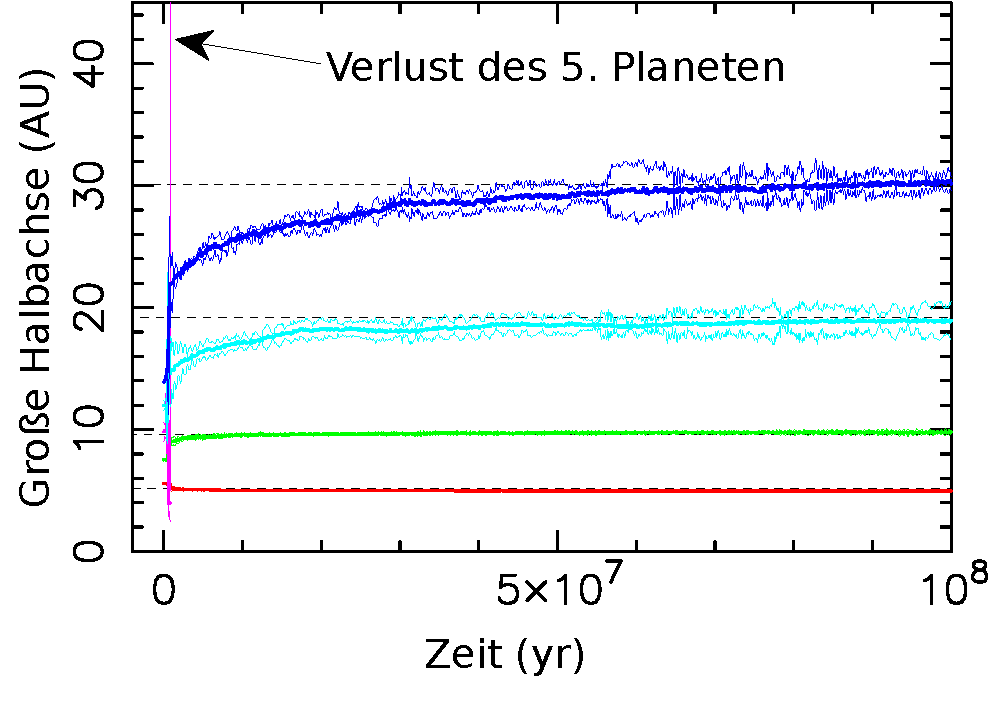
\includegraphics[scale=0.5]{img/Nesvorny2011-1.pdf}
\caption{Zeitliche Entwicklung des Systems, analog zu Abbildung \ref{fig:Orbitalevolution} im Fall mit ursprünglich fünf Riesenplaneten. Man sieht wie einer der Planeten während der Resonanzphase aus dem System geschleudert wird. Bild nach \cite{Nesvorny2011}. }
\label{fig:5planeten}
\end{figure}

Ein mögliche Erweiterung des Nizza-Modells wurde von \cite{Nesvorny2011} vorgeschlagen und später noch weiter vorangetrieben \cite{Nesvorny2012}. Die Idee von Nesvorný war, dass es im Sonnensystem früher womöglich noch mehr Riesenplaneten gegeben hat, diese jedoch während der Instabilitätsphase aus dem Sonnensystem geschleudert wurden (siehe Bild \ref{fig:5planeten}).

\cite{Nesvorny2011} betrachtet multiresonante Ausgangssituationen sowohl mit 1:2 MMR wie im original Nizza-Modell, vor allem aber mit 2:3 MMR zwischen den Gasriesen wie in obigem modifiziertem Nizza-Modell.
Zusätzlich zu Saturn, Jupiter, Uranus und Neptun fügte man bei einigen der Simulationen einen fünften Planeten zwischen Saturn und den Eisriesen ein. Die Masse dieses Planeten entsprach dabei zwischen $3\cdot10^{25}$ und $\unit[3\cdot10^{26}]{kg}$\footnote{Im Paper \cite{Nesvorny2011} scheint sich ein Tippfehler eingeschlichen zu haben, dort steht $\unit{g}$ statt $\unit{kg}$.}, also zwischen einem drittel und der dreifachen Masse der Eisriesen.
Mit hydrodynamischen Simulationen wurde in einem ersten Schritt die wahrscheinlichen Orbits der Planeten bestimmt, anschließend wurde das System mit dem Integrator SyMBA simuliert.
Während die Position des äußeren Rands der Planetesimalscheibe mit $\unit[30]{AU}$ bei der heutigen Position Neptuns gewählt wurde, wurde der innere Rand der Planetesimalscheibe variabel gewählt.
Die Gesamtmasse der Planetesimalscheibe wurde in den Simulationen zwischen $10$ und $\unit[100]{\ME}$ gewählt.
Insgesamt wurden 6000 Simulationen des Systems mit unterschiedlichen Parametern durchgeführt, auf Basis der Ergebnisse erstellte Planetesimalscheibe dann Statistiken, darüber wie Erfolgreich die Simulationen für bestimmte Parameter, insbesondere die Anzahl der Planeten sind.
In der Nachfolgearbeit \cite{Nesvorny2012} wurde der Parameterraum sowie auch die Anzahl der Simulationen noch einmal erhöht. So wurden dabei auch die Anzahl der Planetesimale variiert und auch die Fall mit ursprünglich 6 Riesenplaneten betrachtet. Für jede Anfangsbedingung wurden mindestens 30 bei interessanten Fällen sogar 100 Simulationen durchgeführt, insgesamt wurde fast $10^4$ Simulationen berechnet. Die hohe Anzahl der Berechnungen wurde unter anderem dadurch ermöglicht, dass man die Anfangszustände der Simulationen so wählte, dass es bereits nach sehr kurzer Zeit zur Instabilitätsphase kam.

Für die Bewertung des Erfolgs der Simulationen definierte Nesvorný 4 Kriterien. Kriterium A war, dass das System am Ende genau fünf Riesenplaneten haben muss. Kriterium B beschreibt, dass die großen Halbachsen der Planeten bis auf höchstens 20\% mit den gemessenen Werten übereinstimmen und die Exzentrizitäten und Inklinationen kleiner als 0.11 beziehungsweise $2^\circ$ sind, also nicht höchstens doppelt so groß wie die gemessenen Werte von Saturn beziehungsweise Uranus.
Als drittes Kriterium wurde überprüft, ob Jupiters Orbit so war, dass es zu Begegnungen zwischen ihm und Saturn und einem anderen Planeten kommt, die dazu führen können, dass es zum Einfang von irregulären Satelliten kommt.
Kriterium D beschreibt schließlich ob es zu den in Kapitel \ref{jumpingjupiter} beschriebenen Störungen der Bahnen der Terrestrischen Planeten und des Asteroidengürtels kommt. % invers formulieren?

Leider hat \cite{Nesvorny2012} den Erkenntnisse von \cite{Levison2011}, dass die Berücksichtigung der Wechselwirkungen der Planetesimale untereinander zu einem alternativen Triggermechanismus führt noch nicht berücksichtigt. Auch wurden leider nicht überprüft, ob die Simulationen in Übereinstimmung mit den Eigenschaften des Kupiergürtels sind.

Sie fanden das sich die besten Ergebnisse ergeben, für Systeme mit 5 Riesenplaneten, Planetesimalenscheibenmassen von unter $\unit[50]{\ME}$ und einem Jumping Jupiter\footnote{wobei hier auch der 5 Planet der sein kann der von Jupiter und Saturn gestreut wird}.
Als statistisch vielversprechendstes Szenario haben \cite{Nesvorny2012} folgendes gefunden:
Ein fünfter Riesenplanet mit einer Masse vergleichbar mit der der anderen Eisriesen befand sich Anfangs auf einem Orbit direkt außerhalb der Saturnbahn.
Uranus und Neptun migrieren in die Planetesimalscheibe und zerstreuen diese, dadurch kommt es zur Migration von Jupiter, Saturn und dem fünften Planeten und es kommt zur Instabilität. Der fünfte Planet wird dabei von Jupiter und Saturn gestreut (Jumping Jupiter), kommt aber auch den anderen Planeten nahe. Schließlich wird der fünfte Planet dadurch aus dem System geschleudert.
Somit sind die in Kapitel \ref{jumpingjupiter} beschrieben Probleme gelöst und es kann bei allen Riesenplaneten zum Einfang von irregulären Monden gekommen sein. Somit löst es das Problem das wir im Kapitel \refsec{Monde} hatten, dass das original Nizza-Modell nur die irregulären Mode der Eisriesen vollständig erklären konnte.
Es sei noch erwähnt, dass die Simulationen mit ursprünglich sechs Riesenplaneten zwar weniger erfolgreich waren, als die mit fünf, jedoch immer noch erfolgreicher als die mit nur vier ursprünglichen Riesenplaneten.

Die Erfolgsquote war dabei jedoch relativ gering. Selbst die besten Anfangsbedingungen führten nur in etwa 5\% der Fälle zur Erfüllung aller Kriterien\cite{Nesvorny2012}. Dies ist zwar relativ gering und zeigt, dass -- wenn diesen Modell zutreffen sollte -- unser Sonnensystem kein sehr typisches System ist, man muss jedoch beachten, dass bisher kein anderes Modell diese Eigenschaften überhaupt hat erklären können.
Auch muss man beachten, dass viele der Simulationen zu Ergebnissen führen die mit Leben auf der Erde nicht vereinbar sind. Die Tatsache das wir existieren und uns über solche Modelle Gedanken machen können setzt die habitabilität der Erde voraus, ein Modell auszuschließen weil es im Großteil der Fälle zu einer unbewohnbaren Erde führt ist zumindest fragwürdig\cite{Brasser2009}.

Ein weiterer Vorteil dieser Verallgemeinerungen des Nizza-Modells ist, dass sie eher auf andere Planetensysteme übertragen werden kann. So kann man mit den hier gewonnenen Erkenntnissen auch erklären warum sich die Planeten in Exoplanetensystemen häufig in Resonanz befinden und oft auch hohe Exzentrizitäten haben\cite{Weidenschilling1996,Rasio1996,Marcy2001,Nesvorny2012}.
Darüber hinaus passt die Überlegung ob das Sonnensystem in der Vergangenheit möglicherweise einen oder mehr Planeten verloren hat dazu, dass man inzwischen vermutet, dass es eine sehr große Anzahl an free-floating Planeten, also an Planeten die keinen Stern umkreisen sondern lose durch den interstellaren Raum fliegen gibt. % deutscher Begriff?
Beobachtungen des Mikrolinseneffektes führten dazu, dass \cite{Sumi2011} hochrechneten, dass es möglicherweise fast zweimal so viele freifliegende Planeten in unserem Sonnensystem gibt, als Hauptreihen-Sterne. % Quelle
Somit ist es naheliegen davon auszugehen, dass es eher die Regel als die Ausnahme ist, dass in einem Planetensystem ein oder mehrere Planeten aus dem System geschleudert wird. Es ist also nicht abwegig dies auch im Sonnensystem passiert sein könnte.
Mann muss jedoch darauf hinweisen, dass \cite{Veras2012} gezeigt hat, dass diese große Anzahl an freifliegenden Planeten nicht nur auf diese weise entstanden sein kann.
                                               
\chapter{Zusammenfassende Bewertung}
Das Nizza-Modell stellt ein äußerst erfolgreiches Modell dar. Es stellt das bisher beste Modell zu Erklärung des Sonnensystems dar und kann, wie ich in dieser Arbeit dargelegt habe, zahlreiche Eigenschaften unseres Sonnensystems erklären.
Es erklärt nicht nur die Orbits der Riesenplaneten, sondern auch das Late Heavy Bombardment, die Jupiter- und eventuell auch die Neptun-Trojaner, die irregulären Satelliten und fast alle Eigenschaften des Kuipergürtels.
Kein anderes Modell auf diesem Gebiete hat derartiges erreicht.
Es gibt natürlich aber auch Probleme des Nizza-Modells, sie sind jedoch im Vergleich zu den Erfolgen eher als klein einzustufen und die meisten können -- zumindest potentiell -- durch kleinere Modifikationen des Nizza-Modells behoben werden.
Der besonderer Reiz des Nizza-Modells besteht darin, dass es mit wenigen, plausiblen und klar definierten Anfangsannahmen sehr viele der Eigenschaften des heutigen Sonnensystems erklären kann.
Die neueren Versionen des Modells, können zwar die Erfolge des Nizza-Modells weiter ausbauen und Probleme reduzieren, zahlen dafür jedoch zum einen den Preis eines aufgeweichten und vergrößerten Anfangsparameterraums zum anderen mit niedrigen Erfolgswahrscheinlichkeiten, folglich werden die Aussagen zunehmend statistischer Natur. Dabei zeichnen die Zahlen zumindest auf den ersten Blick ein ernüchterndes Bild, selbst bei den besten Anfangsbedingungen liegen die Erfolgsquoten bestenfalls im einstelligen Prozentbereich.

Hier ist eine vorsichtige und differenzierte Betrachtung der Ergebnisse notwendig. Zum einen dürfen statistische Aussagen nicht überschätzt werden und müssen immer im Kontext gesehen werden. Führen zum Beispiel gewisse Anfangsbedingungen häufiger zum Erfolg, als andere, so heißt das noch nicht notwendigerweise dass erstere Anfangsbedingungen realistischer sind, schließlich betrachtet man immer nur ausgewählte Erfolgsbewertungskriterien. Dazu kommt die schon oben erwähnte Verzerrung durch Negativresultate, die zu einer lebensfeindlichen Erde führen.

Die Absolutwerte der Erfolgswahrscheinlichkeiten hängen von der Stringenz der Erfolgsbewertungskriterien ab. Da man beim Nizza-Modell das $n$-Körperproblem mit hoher Anzahl an Körpern, und dementsprechend vielen Möglichkeiten für die exakten Anfangsbedingungen, über sehr lange Zeiträume hinweg betrachtet, ist es nicht verwunderlich, dass die Erfolgsquoten für immer strenge Erfolgsbewertungskriterien gegen Null gehen.
Da es keinen Grund dafür gibt, dass unser System einen Normalfall darstellt gegen das besonders viele Anfangsbedingungen streben, ist es folglich nicht entscheidend mit wie hoher Wahrscheinlichkeit die von uns ausgewählten Erfolgsbewertungskriterien eintreten, sondern viel mehr die Frage ob das Modell durch Wahl geeigneter Anfangsbedingungen alle wählbaren Kriterien simultan erfüllen kann. % kann fett?
Und genau hier ist das Nizza-Modell und seine Nachfolger äußerst erfolgreich, erfüllt es doch weit mehr Kriterien als alle vorherigen und alternativen Modelle.

Das Nizza-Modell wurde generell erst durch die wachsende Rechenleistung, sowie durch die wesentlich schnelleren symplektischen Simulationsalgorithmen, basierend auf dem besprochenen Algorithmus von \cite{Wisdom1991}, ermöglicht. Dennoch benötigte die Betrachtung der verschiedenen Aspekte des Modells meist speziell optimierte, oft mehrstufige und auf das zu Betrachtende fokussierte Simulationen.
Vielfach wurden dabei auch Vereinfachungen getroffen, von denen sich manche später als problematisch herausgestellt haben; als Beispiel sei hier die Vernachlässigung der Wechselwirkungen zwischen den Planetesimalen genannt. Häufig wurden Vernachlässigungen von Effekten auch als mögliche Erklärung für Diskrepanzen zwischen Modellergebnissen und Realität angeführt.
Dies betrifft insbesondere die Berücksichtigung von Kollisionen, daher glaube ich, dass für die weitere Untersuchung des Nizza-Modells die Entwicklung von Simulationsalgorithmen, die Kollisionen und andere nicht-gravitative Effekte berücksichtigen, von großer Bedeutung ist.
Auch \cite{Morbidelli2002} prognostiziert für die Zukunft eine Entwicklung von reinen numerischen Integratoren zu numerischen Simulatoren, welche nicht nur Newtons Bewegungsgleichungen, sondern eine breite Auswahl an dynamischen und physikalischen Effekten mit berücksichtigt.
Während die Entwicklung des Nizza-Modells in seiner 2005 erschienen Fassung noch wenige Jahre zuvor noch mangels Rechenleistung kaum möglich gewesen wäre, wären auch die neueren Simulationen -- Beispielsweise die von \cite{Nesvorny2012} -- im Jahr 2005 noch lediglich mit sehr großem Aufwand möglich gewesen.
Es ist davon auszugehen das durch die weiter exponentiell wachsende Rechenleistung bereits in wenigen Jahren weitere Durchbrüche ermöglicht werden.
Weiter beschleunigt könnte dies durch neue, noch schnellere Simulationsalgorithmen werden.

Es bleibt die Frage nach dem Wahrheitsgehalt des Modells, denn auch, wenn in den Naturwissenschaften Theorien nicht bewiesen sondern nur falsifiziert werden können, so ist man es doch gewohnt Theorien als bestätigt zu betrachten, wenn sie Falsifikationsversuche -- durch Überprüfung von Vorhersagen des Modells -- überstanden haben.
Dabei hat die Astronomie im allgemeinen das Problem, dass Modelle nicht im Labor aktiv geprüft werden können, sondern man sich auf die vorhandenen beobachteten Systeme beschränken muss.
Im Fall des Nizza-Modells verstärkt sich das Problem, das es sich explizit auf unser Sonnensystem bezieht und es somit nur ein einziges System gibt, dass man analysieren kann.
Wir müssen uns also darauf beschränken immer weitere Eigenschaften unseres Sonnensystems auf Verträglichkeit mit dem Nizza-Modell zu prüfen.
Dies ist jedoch alles andere als trivial, schließlich können oft schon kleine Veränderungen, am Modell oder den Parametern, einen zuvor bestehenden Widerspruch auflösen -- ein Test auf Kompatibilität mit Beobachtungsdaten gibt also entweder ein Hinweis auf Übereinstimmung oder aber die Aussage das entweder das Modell falsch ist oder aber nur noch nicht die richtigen Anfangsbedingung oder Variation des Modells gefunden wurde.
Somit ist das Modell auch nur schwer echt zu falsifizieren. Was bleibt ist die Aussage, dass das Nizza-Modell das erfolgreichste Modell zur Erklärung der Entwicklung unseres Sonnensystems ist das wir bis jetzt kennen.

Das Nizza-Modell stellt einen großen wissenschaftlichen Durchbruch dar, denn es ist damit erstmals möglich, zahlreiche Eigenschaften des Sonnensystems simultan und mit natürlichen Anfangsbedingungen zu erklären. Es ergänzt sich gut mit dem Grad-Track-Modell\cite{Walsh2011}, welches die Entwicklung des inneren Sonnensystems in der Zeit vor dem Auflösen der Gasscheibe beschreibt. Zusammen bilden sie das \glqq Standardmodell\grqq\ der planetaren Evolution des Sonnensystems und sind wissenschaftlich weithin akzeptiert.


%%%% Myr/Gyr einheitlich scheiben
%%%% https://www.youtube.com/watch?v=VXeOh3xmrQM verlinken
%%%% Wie Sumi2011 zitieren?
%%%% Hamilton/Hamiltonian?
%%%% besseres Wort für Planetenbegegnung?
%%%% Bildergrößen vereinheitlichen mit width statt scale
%%%% Vektoren fett!

\newpage

%\chapter{Literaturverzeichnis}

\bibliography{library,libraryKBOmass,libraryoldLHBmodells,libraryoldTrojanermodells,librarysatellites}{}
\bibliographystyle{dinatmod} %gerapali 
%\listoffigures

\cleardoublepage
\backmatter

\pagestyle{empty}
\pagebreak

~\vfill

\noindent
Hiermit versichere ich, dass die am heutigen Tag an der Fakultät für
Physik eingereichte Bachelorarbeit zum
Thema \glqq \thetitle\grqq\ selbstständig
verfasst wurde und, dass ich keine anderen als die angegebenen Quellen und
Hilfsmittel benutzt, sowie Zitate kenntlich gemacht habe.
\vskip 1cm
\noindent
Datum, Unterschrift: \hrulefill


\end{document}
